%----------------------------------------------------------------------------------------
%	PACKAGES AND OTHER DOCUMENT CONFIGURATIONS
%----------------------------------------------------------------------------------------

\documentclass[letterpaper]{article}

\usepackage[utf8]{inputenc} % Required for inputting international characters
% \usepackage[T1]{fontenc} % Output font encoding for international characters
\usepackage[margin=1in]{geometry}
% \usepackage{mathpazo} % Palatino font
\usepackage[spanish]{babel}\decimalpoint % Soporte para español
\usepackage{graphicx} % Paquete para imágenes
\usepackage{fancyhdr} % Paquete para customización de las páginas
\usepackage{lastpage} % Saber última página
\usepackage[hidelinks]{hyperref} % Links para títulos
\usepackage{amsmath}
\usepackage{amssymb}
\usepackage{amsfonts}
\usepackage{xcolor}
\usepackage{empheq}
\usepackage{fancybox}
\usepackage[labelfont=bf]{caption}
\usepackage{array}
\usepackage{float}
\usepackage[most]{tcolorbox}
\usepackage{bookmark}
\usepackage{wrapfig}
\usepackage{multicol}
\usepackage{enumitem}
\usepackage[noend]{algorithm2e}
\usepackage{setspace}
\usepackage{stmaryrd}
\usepackage{ntheorem}
\usepackage{cancel}

\unaccentedoperators

\definecolor{autogray}{RGB}{235,235,235}

\newtcolorbox{greenbox}{
enhanced,
boxrule=0pt,frame hidden,
borderline west={4pt}{0pt}{green!75!black},
colback=green!10!white,
sharp corners
}

\newtcolorbox{redbox}{
enhanced,
boxrule=0pt,frame hidden,
borderline west={4pt}{0pt}{red!75!black},
colback=red!10!white,
sharp corners
}

\newtcolorbox{bluebox}{
enhanced,
boxrule=0pt,frame hidden,
borderline west={4pt}{0pt}{blue!75!black},
colback=blue!10!white,
sharp corners
}

{}\newtcbtheorem[auto counter,number within=section]{ejem}%
  {Ejemplo}{
      fonttitle=\bfseries\upshape, 
    %   fontupper=\slshape,
      arc=0mm, 
      colback=autogray,
      breakable, 
      enhanced jigsaw,
      colframe=gray!75!black}
      {ejemplo}

\newtcbtheorem[auto counter]{theo}%
{Teorema}{fonttitle=\bfseries\upshape, fontupper=\slshape,
    arc=0mm, colback=white,colframe=black!85!white}{theorem}


\pagestyle{fancy} % Definir estilo de páginas
\fancyhf{}
\lhead{\textbf{\scriptsize\rightmark}}
\rhead{\textbf{\footnotesize\leftmark}}
\lfoot{\textbf{\footnotesize IIC3253}}
\cfoot{\textbf{\footnotesize Criptografía y Seguridad Computacional }}
\rfoot{\textbf{\footnotesize Página: \thepage\ de \pageref{LastPage}}}
\setlength{\shadowsize}{2pt}
\setlength{\fboxsep}{5pt}
\setlength\parindent{0pt}
\setlength{\headheight}{19.77605pt}
\setlength{\columnsep}{30pt}
\addtolength{\topmargin}{-4.77605pt}
\bookmarksetup{numbered}
\setlist[itemize]{leftmargin=15pt}
\setlist[enumerate]{leftmargin=15pt}

% Renombre de comandos
\addto\captionsspanish{% Replace "english" with the language you use
  \renewcommand{\contentsname}
    {\LARGE Índice}
}
\addto\captionsspanish{% Replace "english" with the language you use
  \renewcommand{\tablename}
    {Tabla}
}
\renewcommand\arraystretch{1.5}
\renewcommand{\labelitemi}{{\raisebox{.3\height}{\scalebox{0.6}{$\blacklozenge$}}}}
\renewcommand{\headrulewidth}{0.4pt}
\renewcommand{\footrulewidth}{0.4pt}

% Nuevos comandos
\empheqset{marginbox=\psframebox}
\newcommand{\alignformula}[1]{
    \begin{empheq}[box=\shadowbox*]{align*}
        #1
    \end{empheq}\vspace{1pt}
}
\newcommand{\fig}[3]{
    \begin{figure}[H]
        \centering
        \includegraphics[scale=#2]{#1}
        \caption{#3}
        \end{figure}
}
\newcommand{\img}[2]{
    \begin{figure}[H]
        \centering
        \includegraphics[scale=#2]{#1}
        \end{figure}
}
\newcommand{\enlace}[3]{\textcolor{#3}{\textbf{\href{#1}{#2}}}}
\newcommand{\ejemplo}[3]{\begin{ejem}{#1}{#2}#3\end{ejem}\vspace{1pt}}
\newcommand{\teorema}[3]{\begin{theo}{#1}{#2}#3\end{theo}\vspace{1pt}}
\newcommand{\li}[2]{\displaystyle{\lim_{#1 \to #2}}}
\newcommand{\ca}[1]{\mathcal{#1}}
\newcommand{\mbb}[1]{\mathbf{#1}}
\newcommand{\gen}{\texttt{Gen}}
\newcommand{\enc}{\texttt{Enc}}
\newcommand{\dec}{\texttt{Dec}}
\newcommand{\mac}{\texttt{Mac}}
\newcommand{\ver}{\texttt{Verify}}
\newcommand{\ttt}[1]{\texttt{#1}}
\newcommand{\overunder}[3]{\underset{#2}{\overset{#3}{#1}} }

\newcommand\vartextvisiblespace[1][.5em]{%
  \makebox[#1]{%
    \kern.07em
    \vrule height.3ex
    \hrulefill
    \vrule height.3ex
    \kern.07em
  }% <-- don't forget this one!
}

\newcommand{\sbar}{\vartextvisiblespace}

\usepackage{etoolbox}
\apptocmd{\lim}{\limits}{}{}

\begin{document}

%----------------------------------------------------------------------------------------
%	TITLE PAGE
%----------------------------------------------------------------------------------------

\begin{titlepage} % Suppresses displaying the page number on the title page and the subsequent page counts as page 1
    \newcommand{\HRule}{\rule{\linewidth}{0.5mm}} % Defines a new command for horizontal lines, change thickness here

    \center % Centre everything on the page

    %------------------------------------------------
    %	Headings
    %------------------------------------------------

    \textsc{\LARGE Pontificia Universidad Católica de Chile}\\[1.5cm] % Main heading such as the name of your university/college

    \textsc{\Large Departamento de Ciencia de la Computación}\\[0.5cm] % Major heading such as course name

    \textsc{\large Apunte IIC3253}\\[0.5cm] % Minor heading such as course title

    %------------------------------------------------
    %	Title
    %------------------------------------------------

    \HRule\\[0.5cm]

    {\huge\bfseries Criptografía y Seguridad Computacional}\\[0.4cm] % Title of your document

    \HRule\\[1.5cm]

    %------------------------------------------------
    %	Author(s)
    %------------------------------------------------

    \begin{minipage}{0.4\textwidth}
        \begin{flushleft}
            \large
            \textit{Autor}\\
            Cristóbal \textsc{Rojas} % Your name
        \end{flushleft}
    \end{minipage}
    ~
    \begin{minipage}{0.4\textwidth}
        \begin{flushright}
            \large
            \textit{En base a apuntes de}\\
            Prof. Marcelo \textsc{Arenas} \\
            Prof.\,\, Martín \textsc{Ugarte}% Supervisor's name
        \end{flushright}
    \end{minipage}
    ~
    \begin{minipage}{0.8\textwidth}
        \vspace{30pt}
        \begin{center}
            \large
            \textit{En base al texto}\\
            Introduction to Modern Cryptography \\
            J. \textsc{Katz}, Y. \textsc{Lindell}% Supervisor's name
        \end{center}
    \end{minipage}

    % If you don't want a supervisor, uncomment the two lines below and comment the code above
    % {\large\textit{Autor}}\\
    % Cristóbal \textsc{Rojas} % Your name

    %------------------------------------------------
    %	Date
    %------------------------------------------------

    \vfill\vfill\vfill % Position the date 3/4 down the remaining page

    {\large\today} % Date, change the \today to a set date if you want to be precise

    %------------------------------------------------
    %	Logo
    %------------------------------------------------

    \vfill\vfill
    
\includegraphics[width=0.3\textwidth]{img/logo.png}\\[1cm] % Include a department/university logo - this will require the graphicx package

    %----------------------------------------------------------------------------------------

    \vfill % Push the date up 1/4 of the remaining page

\end{titlepage}

% \thispagestyle{empty}
% \begin{redbox}
%     \textbf{Advertencia:} Este no es un documento oficial del curso Cálculo I - MAT1610, el apunte puede presentar fallas y por ende generar error en sus cálculos. Debido a esto, el autor \textbf{no} se hace responsable de cualquier respuesta errónea que pueda dar en alguna prueba, por lo que es su obligación revisar si los contenidos mostrados aquí coinciden con el material oficial del curso. De cualquier manera, como lector está invitado a reportar cualquier falla para así mejorar este apunte cada vez más. Puede enviar un correo a \href{mailto:cristobalrojas@uc.cl}{cristobalrojas@uc.cl}. ¡Muchas gracias!
% \end{redbox}

% \newpage

\thispagestyle{empty}
\pdfbookmark[section]{\contentsname}{toc}
\tableofcontents

\newpage

\section{Introducción}

\subsection{Dos problemas fundamentales: cifrado y autentificación}

La criptografía moderna implica \textit{el estudio de técnicas matemáticas para proteger la información digital, los sistemas y los cálculos distribuidos contra ataques de adversarios}. \medbreak

La seguridad de los \textbf{esquemas criptográficos modernos} (hablaremos de ellos más adelante) recae en una \textbf{llave secreta} compartida con anterioridad entre el emisor (A, de \textit{Alice}) y receptor del mensaje (B, de \textit{Bob}), que debe ser desconocida para algún adversario (E, de \textit{Eavesdropper}). Este escenario, en donde las partes que se comunican comparten alguna información secreta por adelantado, es conocida como \textbf{encriptación de llave privada} (\textit{private-key encryption}). \medbreak

En este contexto, Alice y Bob comparten una llave privada cuando se quieren comunicar en secreto. Uno de ellos, por ejemplo, Alice, puede mandar un \textbf{mensaje} (\textit{plain text}, texto plano) hacia el otro usando la llave para \textbf{encriptar} el mensaje y así obtener un \textbf{texto cifrado} o \textit{cyphertext} que es trasmitido al receptor. Bob, el receptor, usa la misma llave para \textbf{decriptar} el texto cifrado y recuperar el mensaje original.

\fig{img/cap1/1.png}{0.4}{Alice manda un mensaje $m$ a Bob usando una llave privada $k$ que compartieron anteriormente}

La \textbf{autentificación}, en cambio, es el proceso en el que nos interesa garantizar la \textbf{integridad del mensaje} contra un adversario que podría modificar o mandar otros mensajes por el canal de comunicación. \medbreak

Por ejemplo, Alice y Bob, que desean comunicarse de forma autenticada, empiezan por generar y compartir una llave secreta $k$ antes de su comunicación. Cuando una de las partes desea enviar un mensaje $m$ a la otra, calcula una etiqueta (\textit{tag}) $t$ basada en el mensaje y la llave compartida, y envía el mensaje $m$ junto con $t$ a la otra parte. El \textit{tag} se calcula utilizando un \textit{algoritmo de generación de tags} denotado por $\mac$; así, reformulando lo que acabamos de decir, el emisor de un mensaje $m$ calcula $t \leftarrow \mac_k(m)$ y transmite $(m, t)$ al receptor. Al recibir $(m, t)$, la segunda parte verifica si $t$ es un \textit{tag} válido en el mensaje $m$ (con respecto a la llave compartida) o no. Esto se hace ejecutando un \textit{algoritmo de verificación} $\ver$ que toma como entrada la llave compartida, así como un mensaje $m$ y un \textit{tag} $t$, e indica si el \textit{tag} dado es válido. Profundizaremos más sobre este tema en el capítulo X.

\fig{img/cap1/2.png}{0.35}{Alice manda $(m,t)$ a Bob, generando $t$ con $\mac$ y Bob debe verificar $t$ con $\ver$}


\subsection{Sintaxis de encriptación}
Formalmente, un esquema de encriptación de llave privada es definido por un \textbf{espacio de mensajes} $\ca{M}$, un \textbf{espacio de llaves} $\ca{K}$ y un \textbf{espacio de textos cifrados} $\ca{C}$, junto con tres funciones: una para generar llaves ($\gen$), una para encriptar ($\enc$) y otra para decriptar ($\dec$). El espacio de mensajes $\ca{M}$ define el conjunto ``legal'' de mensajes, es decir, los soportados por el esquema. Las funciones del esquema tienen la siguiente funcionalidad:
\begin{itemize}
    \item $\gen$ es un algoritmo de probabilidades que retorna una llave $k$ elegida acorde a una distribución. Es decir, $\gen: \ca{K} \to [0,1]$ tal que
          $$
              \sum_{k\in \ca{K}}\gen(k) = 1
          $$

    \item $\enc$ es una familia de algoritmos de encriptación que toma como input la llave $k$ y el mensaje $m$, y retorna un texto cifrado $c$. Denotamos $\enc_k(m)$ la encriptación del texto plano $m$ usando la llave $k$.
          $$
              \enc = \{ \enc_k \mid k \in \ca{K} \}, \quad \text{con } \enc_k: \ca{M} \to \ca{C}, \;\forall k \in \ca{K}
          $$

    \item $\dec$ es una familia de algoritmos de decriptación que toma como input la llave $k$ y el texto cifrado $c$, y retorna un texto plano $m$. Denotamos $\dec_k(c)$ la decriptación del texto cifrado $c$ usando la llave $k$.
          $$
              \dec = \{ \dec_k \mid k \in \ca{K} \}, \quad \text{con } \dec_k: \ca{C} \to \ca{M}, \;\forall k \in \ca{K}
          $$
\end{itemize}

Un esquema de encriptación debe satisfacer el siguiente requisito de correctitud: para cada llave $k$ generada por $\gen$ y para cada mensaje $m \in \ca{M}$, se tiene que

\alignformula{
    \dec_k(\enc_k(m)) = m
}

En otras palabras, encriptar un mensaje y luego decriptar el texto cifrado resultante usando la misma llave devuelve el mensaje original.

\subsection{Principio de Kerckhoffs}
Si un adversario conoce el algoritmo $\dec$ y la llave $k$ compartida por las dos partes comunicantes, podrá descifrar cualquier texto cifrado transmitido por dichas partes. Por este motivo, las partes comunicantes deben compartir la llave $k$ de forma segura y mantener $k$ completamente oculta para los demás. ¿Quizás también deberían mantener en secreto el algoritmo de descifrado $\dec$? ¿No sería mejor que mantuvieran en secreto todos los detalles del esquema de cifrado? \medbreak

Lo anterior condujo a Auguste Kerckhoffs en 1983 a declarar el siguiente principio:
\begin{center}
    \textit{``La seguridad de un sistema criptográfico \textbf{no} debe depender de que los algoritmos de cifrado y descifrado sean secretos, solo debe depender de que las claves sean secretas''.}
\end{center}

Es decir, un esquema de encriptación debe diseñarse para que sea seguro \textit{incluso} si un espía conoce todos los detalles del esquema, siempre que el atacante no conozca la clave utilizada. Dicho de otro modo, la seguridad no debe depender de que el esquema de cifrado sea secreto; en cambio, el principio de Kerckhoffs exige que la seguridad dependa únicamente del secreto de la clave. \medbreak

Seguimos este principio por tres simples motivos:
\begin{itemize}
    \item Es más fácil mantener la privacidad de una llave que la de un algoritmo.
    \item Si la seguridad se ve comprometida es más fácil cambiar una llave que un algoritmo.
    \item Es mejor usar algoritmos públicos que hayan sido ampliamente verificados.
\end{itemize}

\subsection{Principios de la criptografía moderna}

Podemos mencionar tres grandes principios para la criptografía moderna:
\begin{enumerate}
    \item \textbf{Definiciones formales:} Es importante definir formalmente los sistemas criptográficos y nociones de seguridad usados.
          \begin{center}
              \textit{``Si no sabes lo que quieres conseguir, ¿cómo vas a saber si lo has conseguido?''}
          \end{center}

          Las definiciones formales facilitan esa comprensión al ofrecer una descripción clara de las amenazas que entran en juego y de las garantías de seguridad deseadas. Como tales, las definiciones pueden ayudar a guiar el diseño de esquemas criptográficos. De hecho, es mucho mejor formalizar lo que se necesita \textit{antes} de que comience el proceso de diseño, en lugar de llegar a una definición \textit{post facto} ---posterior a los hechos--- una vez que el diseño se ha completado.

    \item \textbf{Supuestos precisos:} Es importante que los supuestos detrás del funcionamiento de un sistema criptográfico tengan una \textbf{formulación precisa} y sean \textbf{conocidos}. \medbreak

          La mayoría de los esquemas criptográficos modernos no pueden demostrarse seguros de forma incondicional; para ello habría que resolver cuestiones de la teoría de la complejidad computacional que hoy en día parecen lejos de tener respuesta. El resultado de esta desafortunada situación es que las pruebas de seguridad suelen basarse en suposiciones. La criptografía moderna exige que estas suposiciones sean explícitas y precisas desde el punto de vista matemático. En el nivel más básico, esto se debe a que las pruebas de seguridad así lo exigen.

    \item \textbf{Pruebas de seguridad:} Es importante construir \textbf{demostraciones formales de seguridad} (basadas en las definiciones y supuestos). \medbreak

          Los dos principios anteriores que acabamos de describir nos permiten alcanzar nuestro objetivo de proporcionar pruebas rigurosas de que una construcción satisface una definición dada bajo ciertos supuestos. Estas pruebas son especialmente importantes en el contexto de la criptografía, donde hay un atacante que intenta activamente ``romper'' algún esquema. Las pruebas de seguridad ofrecen una garantía irrefutable ---relativa a la definición y los supuestos--- de que ningún atacante tendrá éxito; esto es mucho mejor que adoptar un enfoque sin principios o heurístico del problema. Sin una prueba de que ningún adversario con los recursos especificados puede romper un esquema, sólo nos queda nuestra intuición de que es así. La experiencia ha demostrado que la intuición en criptografía y seguridad informática es desastrosa. Hay innumerables ejemplos de esquemas no probados que se rompieron, a veces inmediatamente y otras años después de ser desarrollados.
\end{enumerate}

\subsection{Seguridad, noción de adversario y tipos de ataque}
En general, una definición de seguridad tiene dos componentes: una \textbf{garantía de seguridad} (o, desde el punto de vista del adversario, lo que constituye un ataque exitoso) y un \textbf{modelo de amenaza} (tipos de ataque). La garantía de seguridad define lo que se pretende que el esquema impida al atacante hacer, mientras que el modelo de amenaza describe el poder del adversario, es decir, qué acciones se supone que el atacante puede llevar a cabo. \medbreak

Los siguientes puntos engloban lo que un esquema de encriptación debería \textbf{garantizar}:
\begin{itemize}
    \item \textit{Debe ser imposible para un adversario recuperar la llave:} aunque la seguridad criptográfica depende de que el adversario no pueda encontrar la llave, este requisito por sí solo no es suficiente para garantizar la seguridad del esquema.
    \item \textit{Debe ser imposible para un adversario recuperar el mensaje (texto plano) a partir del texto cifrado:} este requisito es fundamental para la seguridad del cifrado. Si un adversario puede recuperar el mensaje original a partir del texto cifrado, entonces el esquema de cifrado no es seguro.
    \item \textit{Debe ser imposible para un adversario recuperar cualquier carácter del mensaje a partir del texto cifrado:} este requisito es aún más riguroso, ya que no sólo busca proteger el mensaje completo, sino también la información contenida en él.
    \item \textit{La ``respuesta correcta'': independientemente de la información que tenga el adversario, el texto cifrado no debe filtrar información adicional sobre el mensaje}. Esta definición amplia garantiza que el esquema de cifrado protege la información sin importar cuánta información tenga el adversario. El objetivo del cifrado es evitar que el adversario obtenga cualquier información adicional sobre el mensaje, lo que se logra si el texto cifrado no contiene información adicional más allá de lo que ya se sabe.
\end{itemize}

El \textbf{modelo de amenaza} (los tipos de ataque) especifica qué ``poder'' se supone que tiene el atacante, pero no impone ninguna restricción en la \textit{estrategia} del adversario. Esta es una distinción importante: especificamos lo que asumimos sobre las habilidades del adversario, pero \textbf{no} asumimos nada acerca de cómo usa esas habilidades. Es imposible prever qué estrategias podrían ser utilizadas en un ataque, y la historia ha demostrado que los intentos de hacerlo están destinados al fracaso. Algunos de los tipos de ataque son:
\begin{itemize}
    \item \textbf{Ciphertext-only attack:} es el ataque más básico, en el que el adversario solo observa el texto cifrado y trata de determinar información sobre el texto plano subyacente. Este es el modelo de amenaza que hemos estado asumiendo implícitamente al discutir el esquema de encriptación definido anteriormente.
    \item \textbf{Known-plaintext attack:} aquí, el adversario puede aprender uno o más pares de texto plano/cifrado generados utilizando alguna clave. El objetivo del adversario es deducir información sobre el texto plano subyacente de otro texto cifrado producido utilizando la misma clave.
    \item \textbf{Chosen-plaintext attack:} en este ataque, el adversario puede obtener pares de texto plano/cifrado para textos planos de su elección.
    \item \textbf{Chosen-ciphertext attack:} el último tipo de ataque es aquel en el que el adversario es capaz de obtener (alguna información sobre) el descifrado de textos cifrados de su elección. El objetivo del adversario, una vez más, es aprender información sobre el texto plano subyacente de algún otro texto cifrado (cuyo descifrado el adversario no puede obtener directamente) generado utilizando la misma clave.
\end{itemize}

Aunque los modelos de amenaza están listados en orden de creciente fuerza, ninguno es inherentemente mejor que otro; el adecuado a utilizar depende del entorno en el que se despliega un esquema de encriptación.

\newpage
\section[Criptografía simétrica]{Criptografía simétrica o de clave privada}
Hasta ahora, un ejemplo de criptografía simétrica se ve así:
\img{img/cap2/1.png}{0.35}
Alice desea mandar un mensaje $m$ a Bob, por lo que usa $\enc_k$ para encriptar el mensaje con la llave $k$ que compartieron anteriomente, enviando así el texto cifrado $c$ por un canal de comunicación. Bob, por su lado, puede desencriptar $c$ usando $\dec_k$ con la llave $k$ y así obtener el mensaje $m$. Frente a lo anterior, puede existir un adversario $E$ que quiera conocer la información del mensaje $m$ capturando el texto cifrado $c$.

\subsection{Cifrado del César}
Julio César cifró desplazando (\textit{shift}) las letras del alfabeto 3 lugares hacia delante: \ttt{A} se sustituyó por \ttt{D}, \ttt{B} por \ttt{E}, y así sucesivamente. Al final del alfabeto, las letras se envuelven alrededor y así \ttt{Z} fue reemplazado con \ttt{C}, y con \ttt{B}, y \ttt{X} con \ttt{A}. Por ejemplo, el cifrado del mensaje \ttt{BEGIN THE ATTACK NOW}, con espacios eliminados, da:
$$
    \ttt{EHJLQWKHDWWDFNQRZ}
$$

Un problema inmediato de este cifrado es que el método de encriptación es fijo; \textbf{no hay llave}. Así, \textbf{cualquiera que supiera cómo encriptó César sus mensajes podría desencriptarlos sin esfuerzo}. \medbreak

A pesar de que es poco seguro, este cifrado nos servirá como base para entender OTP, un esquema de encriptación \textit{perfectamente secreto} (ya veremos que significa esto).

\subsection{Una primera versión de One-Time Pad (OTP)}
Veamos una construcción de OTP basada en el cifrado del César. Partimos enumerando las 27 letras del abecedario:
\begin{table}[H]
    \centering
    \ttfamily % aplica la fuente ttfamily para toda la tabla
    \resizebox{\textwidth}{!}{%
        \begin{tabular}{>{\bfseries}c *{27}{c}}
            A & B & C & D & E & F & G & H & I & J & K  & L  & M  & N  & N  & O  & P  & Q  & R  & S  & T  & U  & V  & W  & X  & Y  & Z  \\
            0 & 1 & 2 & 3 & 4 & 5 & 6 & 7 & 8 & 9 & 10 & 11 & 12 & 13 & 14 & 15 & 16 & 17 & 18 & 19 & 20 & 21 & 22 & 23 & 24 & 25 & 26
        \end{tabular}%
    }
\end{table}

Para enviar un mensaje de largo $\ell$, necesitaremos una llave de largo $\ell$. Por ejemplo, probemos mandar el mensaje \ttt{HOLAMUNDO} con la llave \ttt{SECRETKEY}:
\img{img/cap2/2.png}{0.35}

En el ejemplo anterior, a cada letra del mensaje y de la llave, se convierten a un número según la tabla del abecedario, luego se suman y les aplica la operación módulo 27 (ya que son 27 letras). Así, se obtiene un número que representa el cifrado de la letra correspondiente. Es decir:
$$
    \enc_{\ttt{SECRETKEY}}(\ttt{HOLAMUNDO}) = \ttt{ZSNRPÑWHN}
$$
Para desencriptar, hacemos el mismo proceso, solo que en vez de sumar, restamos.
\img{img/cap2/3.png}{0.35}
Y tenemos entonces que
$$
    \dec_{\ttt{SECRETKEY}}(\ttt{ZSNRPÑWHN}) = \ttt{HOLAMUNDO}
$$

Para \textbf{formalizar} este algoritmo, necesitamos convertir mensajes, llaves y textos cifrados en arreglos de enteros:
$$
    \begin{array}{ll}
        m=\ttt{HOLAMUNDO} & \bar{m}=(7,15,11,0,12,21,13,3,15)    \\
        k=\ttt{SECRETKEY} & \bar{k} =(19,4,2,18,4,20,10,4,25)    \\
        c=\ttt{ZSNRPNWHN} & \bar{c} =(26,19,13,18,16,14,23,7,13)
    \end{array}
$$

De la misma forma necesitamos hacer la conversión en la otra dirección:
$$
    a=(4,9,4,12,16,11,15) \quad \bar{a}=\ttt{EJEMPLO}
$$

Naturalmente, vemos que siempre se cumple que $\bar{\bar{s}} = s$. Con esto, definimos OTP en base a
\alignformula{
    \enc_k(m) &= \overline{(\bar{m} + \bar{k}) \bmod 27} \\
    \dec_k(m) &= \overline{(\bar{c} - \bar{k}) \bmod 27}
}

Desde ahora supondremos que nuestros mensajes y llaves \textbf{son arreglos de números}. Con esta suposición en mente, definiremos OTP simplemente usando:
\alignformula{
    \enc_k(m) &= (m + k) \bmod 27 \\
    \dec_k(m) &= (c - k) \bmod 27
}

Con esta definición, vemos entonces que
$$
    \dec_k(\enc_k(m)) = ((m + k) \bmod 27 - k) \bmod 27 = (m + k - k ) \bmod 27 = m \bmod 27 = m
$$

Generalizando, podemos describir $\text{OTP}^{N, \ell}$ sobre $\{0,1,\ldots, N - 1 \}$ y mensajes de largo $\ell$, con:
$$
    \ca{K} = \ca{M} = \ca{C} = \{0,1,\ldots, N - 1 \}
$$

$\gen$ es la \textbf{distribución de probabilidad uniforme} sobre $\{0,1,\ldots, N - 1 \}$, y
\begin{align*}
    \enc_k(m) & =(m+k) \bmod N \\
    \dec_k(c) & =(c-k) \bmod N
\end{align*}

Esperamos que para un esquema criptográfico $(\gen, \enc, \dec)$ se cumpla que
\alignformula{
    \forall k \in \mathcal{K}.\; \forall m \in \mathcal{M}:\quad \dec_k\left(\enc_k(m)\right)=m
}

En este caso diremos que el esquema es \textit{perfectamente correcto}.

\subsection{Perfect secrecy}

Recordemos que un esquema criptográfico está compuesto por una tupla $(\gen, \enc, \dec)$, con un espacio de mensajes $\ca{M}$, un espacio de llaves $\ca{K}$ y un espacio de textos cifrados $\ca{C}$. ¿Cuándo podemos decir que un esquema así es \textit{perfectamente secreto}? Podríamos decir algo como lo siguiente: \textit{``Al ver un texto cifrado $c_0$ pasar, para el atacante el mensaje original $m$ podría haber sido cualquiera''}. \medbreak

¿Cómo formalizamos lo anterior? Dado un texto cifrado $c_0$, se cumple que:
$$
    \forall m_0 \in \ca{M}.\quad \underset{k \sim \gen}{\Pr}[\enc_k(m_0) = c_0] = \frac{1}{|\ca{M}|}
$$

La probabilidad anterior se calcula viendo la probabilidad de haber elegido una llave que encripte $m_0$ como $c_0$:
$$
    \sum_{k\in \ca{K}:\; \enc_k(m_0) = c_0} \gen(k)
$$

Ahora, ¿qué pasa si el atacante tiene información sobre el mensaje? En otras palabras, el atacante posee una distribución de probabilidad $\mathbb{D}$ sobre $\ca{M}$ (conoce la probabilidad de un mensaje). Para cada distribución de probabilidad $\mathbb{D}$ sobre $\ca{M}$ y cada texto cifrado $c_0 \in \ca{C}$ se cumple que:
$$
    \forall m_0 \in \ca{M}: \quad \Pr_{\substack{m \sim \mathbb{D} \\[2pt] k \sim \gen}}\left[m=m_0 \mid \enc_k(m)=c_0\right]=\Pr_{m \sim \mathbb{D}}\left[m=m_0\right]
$$

Recordemos que $\Pr(A \mid B)=\frac{\Pr(A \cap B)}{\Pr(B)}$. Luego, ¿se cumple la siguiente ecuación?
$$
    \frac{\mathbb{D}\left(m_0\right) \sum_{k \in \mathcal{K}: \enc_k\left(m_0\right)=c_0} \gen(k)}{\sum_{m \in \mathcal{M}} \mathbb{D}(m) \sum_{k \in \mathcal{K}: \enc_k(m)=c_0} \gen(k)} \stackrel{?}{=} \mathbb{D}\left(m_0\right)
$$

Para responder la pregunta anterior, volvamos a OTP$^{N,\ell}$ y analicemos si es \textit{perfectamente secreto}.
\begin{enumerate}
    \item $\gen$ es la distribución uniforme $1/N^\ell$.
    \item Para cada $c_0$ y cada $m_0$ existe una única llave $k$ tal que $\enc_k(m_0) = c_0$
\end{enumerate}

Sea $c_0 \in \ca{C}$ un texto cifrado y $m_0$ un mensaje, entonces:
$$
    \frac{\mathbb{D}\left(m_0\right) \sum_{k \in \mathcal{K}: \enc_k\left(m_0\right)=c_0} \gen(k)}{\sum_{m \in \mathcal{M}} \mathbb{D}(m) \sum_{k \in \mathcal{K}: \enc_k(m)=c_0} \gen(k)} = \frac{\mathbb{D}(m_0) \quad \cdot \quad \cancel{1/N^\ell}}{\cancelto{1}{\sum_{m \in \ca{M}}\mathbb{D}(m)} \quad \cdot \quad \cancel{1/N^\ell}} = \mathbb{D}(m_0)
$$

Por lo tanto, \textbf{OTP es un esquema perfectamente secreto} y luego, la ecuación anterior sí se cumple. \medbreak

Como hemos podido ver, \textit{perfect secrecy} es una condición muy fuerte. Lamentablemente, pareciera ser molesto y/o poco razonable que la llave tenga que ser tan larga como el mensaje. ¿Hay alguna forma de modificar OTP para tener $|\ca{K}| < |\ca{M}|$ y seguir teniendo un esquema criptográfico \textit{perfectamente secreto}? Spoiler, no hay tal forma :(

\teorema{}{}{
    Sean $\ca{M}$, $\ca{K}$, $\ca{C}$ espacios de mensajes, llaves y textos cifrados, respectivamente. Si $|\ca{K}| < |\ca{M}|$, entonces no existe un esquema $(\gen, \enc, \dec)$ que sea \textit{perfectamente secreto}.
}

Dado su nombre, podemos decir que OTP solo es seguro solo si \textbf{no} se reutilizan las llaves cada vez que se encripta un mensaje. Si se llega a utilizar la misma llave con la que se cifró el mensaje, OTP \textbf{no es seguro bajo ningún ataque}.

\paragraph*{Demostración teorema.} Supongamos que $|\ca{K}| < |\ca{M}| \leq \ca{C}$ y sea $(\gen, \enc, \dec)$ un esquema criptográfico. Sea $\mathbb{D}$ una distribución sobre $\ca{M}$ y $m_0 \in \ca{M}$ un mensaje tal que $\mathbb{D}(m_0) > 0$. Como $|\ca{K}| < |\ca{M}| \leq \ca{C}$, debe existir $c_0 \in \ca{C}$ para el cual \textbf{ninguna} llave $k \in \ca{K}$ satisface $\enc_k(m_0) = c_0$, por tanto
$$
    \cancelto{0}{\Pr_{\substack{m \sim \mathbb{D} \\ k \sim \gen}} [m = m_0 \mid \enc_k(m_0) = c_0]} \quad < \quad \mathbb{D}(m_0) = \Pr_{m \sim \mathbb{D}} [m = m_0]
$$
\hfill $\blacksquare$

Con todo lo anterior, podemos formalizar la definición de \textit{perfect secrecy} para cualquier esquema criptográfico desde otra perspectiva.

\paragraph*{Definición formal de perfect secrecy.} Un esquema criptográfico $(\gen, \enc, \dec)$ con un espacio de mensajes $\ca{M}$ es \textbf{perfectamente secreto} si para cada distribución de probabilidad para $M$, para cada mensaje $m_0 \in \ca{M}$ y para cada texto cifrado $c \in \ca{C}$ para el cual $\Pr[C = c_0] > 0$:
$$
    \Pr[M = m \mid C = c] = Pr[M = m]
$$
con $M$ y $C$ las variables aleatorias para el mensaje y el texto cifrado.
\paragraph*{Lema.} Un esquema de encriptación $(\gen, \enc, \dec)$ con un espacio de mensajes $\ca{M}$ es perfectamente secreto si, y sólo si se cumple la siguiente ecuación para todo $m, m' \in \ca{M}$ y para todo $c \in \ca{C}$:
$$
    \Pr[\enc_k(m) = c] = \Pr[\enc_k(m') = c]
$$
En otras palabras, la distribución de probabilidad del texto cifrado cuando ciframos $m$ debe ser idéntica a la distribución de probabilidad del texto cifrado cuando se cifra $m'$.

\subsection{Ahora sí, One-Time Pad}

Primero, recordemos que $a \oplus b$ denota el OR-exclusivo (XOR) de dos \textit{strings} binarios de igual longitud $a$ y $b$ (es decir, si $a=a_1 \cdots a_n$ y $b=b_1 \cdots b_n$ son \textit{strings} de $n$ bits, entonces $a \oplus b$ es un \textit{string} de $n$ bits dado por $\left(a_1 \oplus b_1\right) \cdots\left(a_n \oplus b_n\right)$). En OTP, \textbf{la llave} es un \textit{string} uniforme de la \textbf{misma longitud} que el mensaje, y el texto cifrado se calcula simplemente haciendo XORing entre la llave y el mensaje. \medbreak

Antes de hablar de la seguridad de OTP, verifiquemos su \textbf{corrección}: Para cada clave $k$ y cada mensaje $m$ se cumple que $\dec_k\left(\enc_k(m)\right) = \dec_k(k \oplus m) = k \oplus k \oplus m=m$, por lo que OTP constituye un esquema de cifrado válido.
\paragraph*{Construcción del esquema.} Fijemos un entero $n > 0$. El espacio de mensajes $\ca{M}$, el espacio de llaves $\ca{K}$ y el espacio de textos cifrados $\ca{C}$ son todos equivalentes a $\{0,1\}^n$ (el conjunto de todos los \textit{strings} binarios de largo $n$).
\begin{enumerate}
    \item $\gen$: el algoritmo de generación de llaves elige una desde $\ca{K} = \{0,1\}^n$ de acuerdo a la distribución de probabilidad \textbf{uniforme} (es decir, cada uno de los $2^n$ \textit{strings} en el espacio es elegido como llave con probabilidad $1/2^n$).
    \item $\enc$: dada una llave $k \in \{0,1\}^n$ y un mensaje $m \in \{0,1\}^n$, el algoritmo de encriptación retorna el texto cifrado $c = k \oplus m$.
    \item $\dec$: dada una llave $k \in \{0,1\}^n$ y un texto cifrado $c \in \{0,1\}^n$, el algoritmo de decriptación retorna un mensaje $m = k \oplus c$.
\end{enumerate}

\paragraph*{Demostración de la construcción.} Calculamos $\Pr[C = c \mid M = m]$ para un $c \in \ca{C}$ arbitrario y un $m \in \ca{M}$ con $\Pr[M = m] > 0$. Por OTP, tenemos que
$$
    \Pr[C = c \mid M = m] = \Pr[K \oplus m = c \mid M = m] = \Pr[K = m \oplus c \mid M = m] = \frac{1}{2^n}
$$
donde $M$, $K$ y $C$ son las variables aleatorias para el mensaje, la llave y el texto cifrado, que son \textbf{independientes} entre sí. Aquí, la primera ecuación es por definición del esquema y el hecho que condicionamos el evento de que $M = m$, y la última ecuación es válida porque la llave $K$ es un $n$-bit uniforme  que es independiente de $M$. Fijemos cualquier distribución de probabilidad sobre $\ca{M}$. Usando el resultado de arriba, vemos que para cualquier $c \in \ca{C}$ tenemos:
$$
    \Pr[C = c] = \sum_{m \in \ca{M}} \Pr[C = c \mid M = m]\cdot \Pr[M = m] = \frac{1}{2^n} \cdot \sum_{m \in \ca{M}} \Pr[M = m] = \frac{1}{2^n}
$$
donde la suma es sobre $m \in \ca{M}$ con $\Pr[M = m] \neq 0$. Por el Teorema de Bayes:
$$
    \Pr[M = m \mid C = c] = \frac{\Pr[C = c \mid M = m] \cdot \Pr[M = m]}{\Pr[C = c]} = \frac{2^{-n} \cdot \Pr[M = m]}{2^{-n}} = \Pr[M = m]
$$
Concluimos entonces que OTP es \textit{perfectamente secreto}. \hfill $\blacksquare$

\subsection{Permutaciones pseudo-aleatorias (PRP)}
Recordemos que una noción de seguridad debe incluir:
\begin{itemize}
    \item Un modelo de amenaza (tipos de ataque), que define las capacidades de un \textbf{adversario}.
    \item Una garantía de seguridad, lo cual normalmente se traduce en definir qué significa que el adversario no tenga éxito en su ataque.
\end{itemize}

Vamos a definir una primera noción de seguridad que nos va a permitir mostrar que OTP no es seguro si la llave es \textbf{reutilizada}, como mencionamos anteriormente. \medbreak

Consideremos un largo $n$ fijo tal que los espacios de mensajes, llaves y textos cifrados cumplen que $\ca{M} = \ca{K} = \ca{C} = \{0,1\}^n$ y $(\gen, \enc, \dec)$ es un esquema criptográfico. Veamos un \textbf{juego} para definir una \textbf{pseudo-random permutation} (PRP):
\begin{enumerate}
    \item Un \textbf{verificador} elige $b \in \{0,1\}$ con distribución uniforme (por ejemplo, tirar una moneda).
          \begin{enumerate}
              \item[1.1.] Si $b = 0$, entonces elige una clave $k \in \ca{K}$ según la distribución $\gen$ y define $f(x) = \enc_k(x)$.
              \item[1.2.] Si $b = 1$, entonces elige una permutación $\pi$ con distribución uniforme y define $f(x) = \pi(x)$
          \end{enumerate}
    \item El \textbf{adversario} elige una palabra $y \in \{0,1\}^n$ y el verificador responde con $f(y)$.
    \item El paso 2. es repetido $q$ veces.
    \item El adversario indica si $b = 0$ o $b = 1$, y gana si su elección es correcta.
\end{enumerate}

La probabilidad de que el adversario gane depende de la cantidad de rondas $q$. Si el adversario ``tira una moneda'' en el paso 4., entonces su probabilidad de ganar es $\frac{1}{2}$.

\paragraph{Definición de PRP.} Decimos que $(\gen, \enc, \dec)$ es una permutación pseudo-aleatoria si \textbf{no existe} un adversario que pueda ganar el juego con una probabilidad significativamente mayor a $\frac{1}{2}$. \medbreak

No imponemos restricciones en las capacidades computacionales del adversario, podríamos tener una noción más débil donde el adversario puede realizar una cantidad de operaciones que es polinomial en $n$. Por ejemplo, solo puede realizar $n^2$ operaciones. Debemos entonces definir qué significa que \textit{la probabilidad de ganar el juego sea significativamente mayor a} $\frac{1}{2}$ (podría ser $\frac{3}{4}$, por ejemplo). También, tenemos que indicar cuál es el número de rondas $q$.

\paragraph{Un primer ejemplo.} Considere un esquema $(\gen, \enc, \dec)$ tal que:
\begin{itemize}
    \item $\gen(k_0) = 1$ para una llave fija $k_0 \in \ca{K}$.
    \item $\gen(k) = 0$ para todo $k \in \ca{K}$ tal que $k \neq k_0$.
\end{itemize}
Vamos a demostrar que este esquema criptográfico no es una PRP con una ronda ($q = 1$). La estrategia del adversario es la siguiente:
\begin{itemize}
    \item En el paso 2. toma $y = 0^n$ y recibe $f(y)$ como respuesta del verificador.
    \item Si $f(y) = \enc_{k_0}(y)$ entonces indica que $b = 0$, si no, indica que $b = 1$.
\end{itemize}
¿Puede el adversario equivocarse al indicar el valor de $b$? ¿Cuál es la probabilidad de que gane el juego? Veamos. Definamos $A$ como el evento ``Adversario gana el juego'', entonces:
\begin{align*}
    \Pr[A] & = \Pr[A \mid b = 0] \cdot \Pr[b = 0] + \Pr[A \mid b = 1] \cdot \Pr[b = 1]   \\
           & = \Pr[A \mid b = 0] \cdot \frac{1}{2} + \Pr[A \mid b = 1] \cdot \frac{1}{2}
\end{align*}
Vemos que:
\begin{itemize}
    \item $\Pr[A \mid b = 0] = 1$
    \item $\Pr[A \mid b = 1] = \Pr[\pi(y) \neq \enc_{k_0}(y)]$

          En este caso el verificador elige una permutación $\pi: \{0,1\}^n \to \{0,1\}^n$ con \textbf{distribución uniforme}. Si $\pi(y) = \enc_{k_0}(y)$, entonces el adversario da la respuesta equivocada. Luego,
          \begin{align*}
              \Pr[\pi(y) \neq \enc_{k_0}(y)] & = 1 - \Pr[\pi(y) = \enc_{k_0}(y)]                          \\
                                             & = 1 - \frac{\text{casos favorables}}{\text{casos totales}} \\
                                             & = 1 - \frac{(2^n - 1)!}{(2^n)!}                            \\
                                             & = 1 - \frac{1}{2^n}
          \end{align*}
\end{itemize}
De la ecuación anterior:
\begin{itemize}
    \item \textbf{Casos totales:} número de permutaciones $\pi: \{0,1\}^n \to \{0,1\}^n$.
    \item \textbf{Casos favorables:} número de permutaciones $\pi: \{0,1\}^n \to \{0,1\}^n$ tales que $\pi(0^n)$ es igual al valor fijo $\enc_{k_0}(0^n)$.
\end{itemize}

Finalmente, tenemos que
\begin{align*}
    \Pr[A] & = \Pr[A \mid b = 0] \cdot \frac{1}{2} + \Pr[A \mid b = 1] \cdot \frac{1}{2} \\
           & = 1 \cdot \frac{1}{2} + \left(1 - \frac{1}{2^n}\right) \cdot \frac{1}{2}    \\
           & = 1 - \frac{1}{2^{n+1}}
\end{align*}

Por ende, el adversario \textbf{sí} gana el juego con probabilidad significativamente mayor a $\frac{1}{2}$. Puede verificar este hecho tomando $n = 10$ o $n = 100$.

\paragraph{Un segundo ejemplo.} Dado que $\ca{M} = \ca{K} = \ca{C} = \{0,1\}^n$, debemos realizar las operaciones de OTP en módulo 2:
\img{img/cap2/4.png}{0.25}

Veremos que OTP no es una PRP con dos rondas. La estrategia del adversario es la siguiente:
\begin{itemize}
    \item En el paso 2. toma $y_1 = 0^n$ e $y_2 = 1^n$, y recibe $f(y_1)$ y $f(y_2)$ como respuesta del verificador.
    \item Si $y_2 + f(y_1) = f(y_2)$ entonces indica que $b = 0$, sino indica que $b = 1$.
\end{itemize}

Si $b = 0$, el verificador está usando OTP y existe una clave $k$ tal que:
\begin{align*}
    y_1 + k & = f(y_1) \\
    y_2 + k & = f(y_2)
\end{align*}

Como $y_1 = 0^n$, se tiene que $k = f(y_1)$ (sumamos 0 en binario), y se concluye que $y_2 + f(y_1) = f(y_2)$. Luego, consideremos nuevamente el evento $A$ como ``Adversario gana el juego'', entonces, la probabilidad de ganar el juego con dos rondas es la siguiente:
\begin{align*}
    \Pr[A] & = \Pr[A \mid b = 0] \cdot \Pr[b = 0] + \Pr[A \mid b = 1] \cdot \Pr[b = 1]   \\
           & = \Pr[A \mid b = 0] \cdot \frac{1}{2} + \Pr[A \mid b = 1] \cdot \frac{1}{2}
\end{align*}
Vemos que:
\begin{itemize}
    \item $\Pr[A \mid b = 0] = 1$
    \item $\Pr[A \mid b = 1] = \Pr[\pi(y_2) \neq y_2 + \pi(y_1)]$

          En este caso, el verificador elige una permutación $\pi:\{0,1\}^n \to \{0,1\}^n$ con \textbf{distribución uniforme}. Si $\pi(y_2) = y_2 + \pi(y_1)$, entonces el adversario da la respuesta equivocada. Así, vemos que:
          \begin{align*}
              \Pr[\pi(y_2) \neq y_2 + \pi(y_1)] & = 1 - \Pr[\pi(y_2) = y_2 + \pi(y_1)]                       \\
                                                & = 1 - \frac{\text{casos favorables}}{\text{casos totales}} \\
                                                & = 1 - \frac{2^n \cdot (2^n - 2)!}{(2^n)!}                  \\
                                                & = 1 - \frac{1}{2^n - 1}
          \end{align*}
\end{itemize}
De la ecuación anterior:
\begin{itemize}
    \item \textbf{Casos totales:} número de permutaciones $\pi:\{0,1\}^n\to\{0,1\}^n$.
    \item \textbf{Casos favorables:} número de permutaciones $\pi:\{0,1\}^n\to\{0,1\}^n$ tales que $\pi(1^n) = 1^n + \pi(0^n)$.
\end{itemize}
Finalmente, tenemos que
\begin{align*}
    \Pr[A] & = \Pr[A \mid b = 0] \cdot \frac{1}{2} + \Pr[A \mid b = 1] \cdot \frac{1}{2}  \\
           & = 1 \cdot \frac{1}{2} + \left(1 - \frac{1}{2^n - 1}\right) \cdot \frac{1}{2} \\
           & = 1 - \frac{1}{2 \cdot (2^n - 1)}
\end{align*}
Por ende, el adversario gana el juego con una probabilidad significativamente mayor a $\frac{1}{2}$, y entonces OTP no es una PRP con dos rondas.

% \section[Autentificación]{Definiciones y herramientas para la autentificación}

\subsection{Funciones de hash}

\paragraph{Definición.} Las funciones de hash \textbf{criptográficas} son funciones de un espacio de posibles mensajes a un espacio de mensajes de largo fijo:
$$
    h: \ca{M} \to \ca{H}
$$

$\ca{M}$ es el espacio de mensajes y $\ca{H}$ es el espacio de posibles valores de la función de hash. Por ejemplo:
$$
    \ca{M} = \{0,1\}^n \quad \text{y} \quad \ca{H} = \{0,1\}^{128}
$$
Decimos que $h(m)$ es el hash de un mensaje $m$. \medbreak

\paragraph{Resistencia a preimágenes.} Una propiedad básica de las funciones de hash es que debe existir un algoritmo \textbf{eficiente}, tal que dado un mensaje $m \in \ca{M}$, calcula $h(m)$. Además, no debe existir un algoritmo eficiente que, dado $x \in \ca{H}$, encuentra $m \in \ca{M}$ tal que $h(m) = x$. Esta propiedad se denota como ser resistente a preimagen.

\paragraph{¿Funciones criptográficas?} Insistimos en el adjetivo criptográficas ya que estas funciones deben ser construidas para ser seguras y soportar ataques de adversarios, en la medida que sea posible. Por ejemplo, consideremos la siguiente función de hash:
$$
    h(m) = (A \cdot m + B) \bmod C
$$

Suponemos que los mensajes son números naturales y que $A$, $B$ y $C$ son constantes, con $C$ un número primo. ¿Es esta función resistente a preimagen? Digamos que $h(m) = (13 \cdot m + 97) \bmod 641$. ¿Podemos encontrar un mensaje $m$ tal que $h(m) = 200$? Una combinación de herramientas de aritmética modular nos pueden dar una respuesta rápida:
$$
    h(501) = (13 \cdot 501 + 97) \bmod 641 = 200
$$

Concluimos entonces que $h$ \textbf{no} es resistente a preimágenes.

\paragraph{Resistencia a colisiones.} Otra propiedad de las funciones de hash es que no debe existir un algoritmo eficiente que pueda encontrar $m_1, m_2 \in \ca{M}$ tales que $m_1 \neq m_2$ y $h(m_1) = h(m_2)$. Esta propiedad se denota como ser resistente colisiones.

\paragraph{Definición formal.} Una función de hash es un par $(\gen, h)$ tal que:
\begin{itemize}
    \item $\gen$ es un algoritmo aleatorizado de tiempo polinomial. $\gen$ toma como entrada un parámetro de seguridad $1^n$ y genera una llave $s$.
    \item $h$ es un algoritmo de tiempo polinomial, que toma como entrada $s$ y un mensaje $m \in \{0,1\}^*$, y retorna un hash $h^s(m) \in \{0,1\}^{\ell(n)}$, donde $\ell$ es un polinomio fijo.
\end{itemize}

Si $m \in \{0,1\}^{\ell'(n)}$ para un polinomio fijo $\ell'$ tal que $\ell'(n) > \ell(n)$, entonces $(\gen, h)$ es una función de hash de \textbf{largo fijo}.

\paragraph{Funciones despreciables.} Sea $\mathbb{R}^+$ el conjunto de los números reales positivos, y $\mathbb{R}_0^+ = \mathbb{R}^+ \cup \{0\}$. Una función $f: \mathbb{N} \to \mathbb{R}_0^+$ es \textbf{despreciable} si:
\alignformula{
    \forall \text{ polinomio } p: \mathbb{N} \to \mathbb{R}.\; \exists n_0 \in \mathbb{N}.\; \forall n \geq n_0. \; f(n) < \frac{1}{p(n)}
}
\begin{itemize}
    \item Por ejemplo, las funciones $f(n) = 2^{-n}$ y $f(n) = n^{-\log(n)}$ son funciones despreciables.
    \item Si $f$ y $g$ son funciones despreciables y $p$ es un polinomio, entonces $f + g$ y $f \cdot p$ son funciones despreciables.
\end{itemize}

\paragraph{Formalizando la resistencia a colisiones.} Considere una función de hash $(\gen, h)$. Definimos el juego $\texttt{Hash-Col}(n)$:
\begin{enumerate}
    \item El verificador genera $s = \gen(1^n)$ y se lo entrega al adversario.
    \item El adversario elige mensajes $m_1$ y $m_2$ con $m_1 \neq m_2$.
    \item El adversario gana el juego si $h^s(m_1) = h^s(m_2)$, en caso contrario, pierde.
\end{enumerate}

Una función de hash $(\gen, h)$ se dice resistente a colisiones si \textbf{para todo adversario que funciona como un algoritmo aleatorizado de tiempo polinomial}, existe una función despreciable $f(n)$ tal que:
\alignformula{
    \Pr[\text{Adversario gane } \texttt{Hash-Col}(n)] \leq f(n)
}

Como colorario de esta definición, si una función de hash es resistente a colisiones, entonces es resistente a preimágen.

\subsection{Códigos de autentificación de mensajes (MAC)}
\fig{img/cap3/1.png}{0.25}{Escenario de autentificación de mensajes}

Un objetivo básico de la criptografía es permitir que las partes se comuniquen de manera segura. Pero, ¿qué implica que ``la comunicación sea segura''? Antes, mostramos cómo es posible lograr \textit{perfect secrecy}; es decir, cómo se puede utilizar la encriptación para evitar que un adversario aprenda algo sobre los mensajes enviados a través de un canal público. Sin embargo, no toda la encriptación se relaciona con \textit{perfect secrecy}, y no todos los adversarios se limitan a solo leer mensajes encriptados que pasan por el canal. En muchos casos, es de igual o mayor importancia garantizar la integridad del mensaje (o la autenticación del mensaje) contra un adversario que puede introducir mensajes en el canal o modificar mensajes en tránsito.

\paragraph{Encriptación vs. autentificación.} Mantener un mensaje secreto y mantener la integridad de un mensaje son objetivos distintos, y por ende también lo son las técnicas y herramientas para lograr cada una de esas tareas. Desafortunadamente, mantener un mensaje secreto y la integridad del mismo a menudo se confunden y se entrelazan innecesariamente, así que seamos claros desde el principio: la encriptación no proporciona (en general) ninguna integridad, y \textbf{no se debe suponer que la encriptación garantiza la autenticación del mensaje} a menos que esté específicamente diseñada con ese propósito en mente.

\paragraph{Definiciones para MAC.} Dado el problema anterior, necesitamos un mecanismo que ayude a las partes comunicantes a saber si el mensaje que se ha enviado a sido manipulado o no. La herramienta para esto son los \textit{códigos de autentificación de mensajes} (MAC). Ahora, tendremos un espacio de llaves $\ca{K}$, un espacio de mensajes $\ca{M}$ y un espacio de \textbf{tags} $\ca{T}$, con los que definimos el esquema de autentificación de mensajes $(\ttt{Gen}, \ttt{Mac}, \ttt{Vrfy})$ tal que:

\begin{itemize}
    \item $\ttt{Gen}$ es un algoritmo de generación de llaves que recibe un \textbf{parámetro de seguridad} $1^n$ y retorna una llave $k$, con $|k| \geq n$.
    \item $\ttt{Mac}$ es una familia de funciones:
    $$
    \ttt{Mac} = \{\ttt{Mac}_k \mid k \in \ca{K}\}, \quad \text{con } \ttt{Mac}_k:\ca{M} \to \ca{T}, \forall k \in \ca{K}
    $$
    Es decir, es un algoritmo de generación de tags. Recibe un mensaje $m$ y una llave $k$ y retorna un tag $t$. Denotamos esto como $t = \ttt{Mac}_k(m)$
    \item $\ttt{Vrfy}$ es una familia de funciones: 
    $$
    \ttt{Vrfy} = \{\ttt{Vrfy}_k \mid k \in \ca{K}\}, \quad \text{con } \ttt{Vrfy}_k:\ca{M} \times \ca{T} \to \{0,1\}, \forall k \in \ca{K}
    $$
    Es decir, es un algoritmo de verificación. Recibe una llave $k$, un mensaje $m$ y un tag $t$. Retorna un bit $b$, con $b = 1$ un mensaje válido y $b = 0$ un mensaje inválido. Denotamos esto como $b = \ttt{Vrfy}_k(m, t)$.
\end{itemize}

\paragraph*{Requisito para MAC.} En un esquema de autentificación de mensajes $(\ttt{Gen}, \ttt{Mac}, \ttt{Vrfy})$ es necesario que para todo $n$, para toda llave $k \in \ca{K}$ que retorna $\ttt{Gen}(1^n)$  y para cada mensaje $m \in \ca{M}$, se cumpla que:
\alignformula{
\ttt{Vrfy}_k(m, \ttt{Mac}_k(m)) = 1
}
\paragraph{Juego para MAC.} Un atacante puede romper el esquema de autentificación si logra generar una un tag falso, es decir, si produce un mensaje $m$ junto con una etiqueta $t$ tal que:
\begin{enumerate}
    \item $t$ es una etiqueta válida para el mensaje $m$ (es decir, $\ttt{Vrfy}_k(m,t) = 1$), y
    \item las partes comunicantes no habían autenticado previamente $m$.
\end{enumerate}
Estas condiciones implican que si el adversario enviara $(m,t)$ a una de las partes comunicantes, entonces esa parte sería engañada erróneamente pensando que $m$ se originó en la otra parte legítima (ya que $\ttt{Vrfy}_k (m, t) = 1$) aunque no fue así. \bigbreak

Decimos que MAC es \textit{inmune a falsificación (existentially unforgeable)} cuando el adversario es incapaz de falsificar un tag válido para cualquier mensaje. En base a esto, podemos definir el juego $\ttt{Forge}_{\ttt{Mac}}(n)$:
\begin{enumerate}
    \item El verificador invoca $\gen(1^n)$ para generar una llave $k$, con $n$ el parámetro de seguridad.
    \item El adversario envía $m_0 \in \ca{M}$ al verificador.
    \item El verificador responde $\mac_k(m_0)$.
    \item Los pasos 2 y 3 se repiten tantas veces como quiera el adversario.
    \item El adversario envía $(m,t)$, siendo $m$ un mensaje que no había enviado antes.
\end{enumerate}
Decimos que el adversario \textbf{gana} el juego si se cumple que $\ver_k(m, t) = 1$, y pierde en caso contrario.

\paragraph{Seguridad de MAC.} Decimos que un código de autentificación de mensajes MAC es inmune a falsificación, o en otras palabras, es \textbf{seguro}, si todo adversario $A$ que juega $\ttt{Forge}_{\mac}(n)$ en tiempo polinomial en $n$ tiene una probabilidad despreciable de ganar el juego, es decir:
\alignformula{
    \Pr[A \text{ gane } \ttt{Forge}_{\mac}(n)] \leq f(n)
}
con $f(n)$ una función despreciable.
\paragraph{Replay attacks.} Los códigos de autenticación de mensajes no ofrecen protección contra \textit{replay attacks} (ataques de repetición), en los que un atacante reenvía un mensaje previamente autenticado con su etiqueta válida. Aunque son una amenaza importante, un MAC no puede proteger contra estos ataques, ya que \textbf{no está diseñado para resistirlos}. La protección debe ser manejada a nivel de aplicación, ya que la decisión de si un mensaje repetido debe ser tratado como ``válido'' puede depender de la misma aplicación como tal.

% \section{Lenguajes libres de contexto}

\subsection{Gramáticas libres de contexto}

\subsubsection{Gramáticas}

\paragraph{Definición.} Una \textbf{gramática libre de contexto} (CFG) es una tupla:
\alignformula{
    \ca{G} = (V, \Sigma, P, S)
}
\begin{itemize}
    \item $V$ es un conjunto finito de \textbf{variables} o \textbf{no-terminales}.
    \item $\Sigma$ es el alfabeto finito (o \textbf{terminales}) tal que $\Sigma \cap V = \varnothing$.
    \item $P \subseteq V \times(V \cup \Sigma)^*$ es un subconjunto finito de \textbf{reglas} o \textbf{producciones}.
    \item $S \in V$ es la \textbf{variable inicial}.
\end{itemize}

\ejemplo{}{}{
    Considere la gramática $\ca{G} = (V, \Sigma, P, S)$ tal que:
    \begin{itemize}
        \item $V = \{X, Y\}$
        \item $\Sigma = \{a,b\}$
        \item $\{(X, aXb), (X, Y), (Y, \epsilon)\}$
        \item $S = X$
              \begin{align*}
                  \ca{G}: \quad  X & \to aXb      \\
                  X                & \to Y        \\
                  Y                & \to \epsilon
              \end{align*}
    \end{itemize}
}

\paragraph{Notación.} En este texto:
\begin{itemize}
    \item Para las \textbf{variables} en una gramática usaremos letras mayúsculas: $X,Y,Z,A,B,C,\ldots$
    \item Para los \textbf{terminales} en una gramática usaremos letras minúsculas: $a,b,c,\ldots$
    \item Para palabras en $(V \cup \Sigma)^*$ usaremos símbolos: $\alpha, \beta, \gamma, \ldots$
    \item Para una producción $(A,\alpha) \in P$ la escribimos como: $A \to \alpha$
\end{itemize}

\paragraph{Simplificación.} Si tenemos un conjunto de reglas de la forma:
$$
    \begin{array}{lll}
        X & \rightarrow & \alpha_1 \\
        X & \rightarrow & \alpha_2 \\
          & \cdots      &          \\
        X & \rightarrow & \alpha_n
    \end{array}
$$
entonces escribimos estas reglas \textbf{sucintamente} como
$$
    X \to \alpha_1 \mid \alpha_2 \mid \cdots \mid \alpha_n
$$
Recordando que $\alpha_1, \alpha_2, \ldots, \alpha_n \in (V \cup \Sigma)^*$.

\ejemplo{}{}{
    La gramática del ejemplo anterior:
    \begin{align*}
        \ca{G}: \quad  X & \to aXb      \\
        X                & \to Y        \\
        Y                & \to \epsilon
    \end{align*}
    Podemos escribirla en notación \textbf{sucinta} como:
    \begin{align*}
        \ca{G}: \quad X & \to aXb \mid Y \\
        Y               & \to \epsilon
    \end{align*}
}

\paragraph{Producciones.} Sea $\ca{G}$ una CFG. Definimos la relación $\Rightarrow \subseteq(V \cup \Sigma)^* \times(V \cup \Sigma)^*$ de \textbf{producción} tal que:
\alignformula{
    \alpha \cdot X \cdot \beta \Rightarrow \alpha \cdot \gamma \cdot \beta \quad \text { si, y solo si, } \quad(X \rightarrow \gamma) \in P
}
para todo $X \in V$ y $\alpha, \beta, \gamma \in(V \cup \Sigma)^*$. \medbreak

Si $\alpha X \beta \Rightarrow \alpha \gamma \beta$ entonces decimos que:
\begin{itemize}
    \item $\alpha X \beta$ \textbf{produce} $\alpha \gamma \beta$ o
    \item $\alpha \gamma \beta$ \textbf{es producible} desde $\alpha X \beta$.
    \item $\alpha X \beta \Rightarrow \alpha \gamma \beta$ es \textbf{reemplazar} $\gamma$ en $X$ en la palabra $\alpha X \beta$.
\end{itemize}

\paragraph{Derivaciones.} Sea $\ca{G}$ una CFG. Dadas dos palabras $\alpha, \beta \in(V \cup \Sigma)^*$ decimos que $\alpha$ \textbf{deriva} $\beta$:
\alignformula{
    \alpha \overunder{\Rightarrow}{}{*} \beta
}
si existe $\alpha_1, \alpha_2, \ldots, \alpha_n \in(V \cup \Sigma)^*$ tal que: $\alpha \Rightarrow \alpha_1 \Rightarrow \alpha_2 \Rightarrow \ldots \Rightarrow \beta$, con $\overunder{\Rightarrow}{}{*}$ la \textbf{clausura refleja y transitiva} de $\Rightarrow$, esto es:
\begin{enumerate}
    \item $\alpha \overunder{\Rightarrow}{}{*} \alpha$
    \item $\alpha \overunder{\Rightarrow}{}{*} \beta$ si, y sólo si, existe $\gamma$ tal que $\alpha \overunder{\Rightarrow}{}{*} \gamma$ y $\gamma \Rightarrow \beta$.
\end{enumerate}
para todo $\alpha, \beta \in (V \cup \Sigma)^*$. Notemos que $\Rightarrow$ y $\overunder{\Rightarrow}{}{*}$ son relaciones entre palabras en $(V \cup \Sigma)^*$.

\paragraph{Lenguaje.} Sea $\ca{G}$ una CFG. El \textbf{lenguaje} de una gramática $\ca{G}$ se define como:
\alignformula{
    \mathcal{L}(\mathcal{G})=\left\{w \in \Sigma^* \mid S \stackrel{\star}{\Rightarrow} w\right\}
}

$\ca{L}(\ca{G})$ son todas las palabras en $\Sigma^*$ que se pueden derivar desde $S$.

\ejemplo{}{}{
    Sea $\ca{G}$ una CFG tal que:
    \begin{align*}
        \ca{G}: \quad X & \to aXb \mid Y \\
        Y               & \to \epsilon
    \end{align*}
    \begin{itemize}
        \item Como $X \overunder{\Rightarrow}{}{*} aaabbb$, entonces $aaabbb \in \ca{L}(\ca{G})$.
        \item En general, uno puede demostrar por \textbf{inducción} que:
              $$
                  \mathcal{L}(\mathcal{G})=\left\{a^n b^n \mid n \geq 0\right\}
              $$
    \end{itemize}
}

\paragraph{Lenguaje libre de contexto.} Diremos que $L \subseteq \Sigma^*$ es un \textbf{lenguaje libre de contexto} si, y sólo si, existe una gramática libre de contexto $\ca{G}$ tal que:
\alignformula{
    L = \ca{L}(\ca{G})
}

\ejemplo{}{}{
    Los siguientes son lenguajes libres de contexto:
    \begin{itemize}
        \item $L=\left\{a^n b^n \mid n \geq 0\right\}$
        \item $\text{Par}=\left\{w \in\{a, b\}^* \mid w \text { tiene largo par }\right\}$
        \item $\text{Pal}=\left\{w \in\{a, b\}^* \mid w=w^{\mathrm{rev}}\right\}$
    \end{itemize}
}

\subsubsection{Árboles y derivaciones}

\paragraph{Definición.} El conjunto de \textbf{árboles ordenados y etiquetados} (o solo árboles) sobre etiquetas $\Sigma$ y $V$, se define recursivamente como:
\begin{itemize}
    \item $t:=a$ es un árbol para todo $a \in \Sigma$.
    \item si $t_1,\ldots, t_k$ son árboles, entonces $t:= X(t_1, \ldots, t_k)$ es un árbol para todo $X \in V$.
\end{itemize}

Para un árbol $t = X(t_1,\ldots,t_k)$ cualquiera se define:
\begin{itemize}
    \item $\texttt{raiz}(t)=X$
    \item $\texttt{hijos}(t)= t_1,\ldots,t_k$
\end{itemize}

Si $t = a$, entonces decimos que $t$ es una \textbf{hoja}, $\texttt{raiz}(t) = a$ y $\texttt{hijos}(t) = \epsilon$.

\paragraph{Definición.} Fije una CFG $\ca{G} = (V, \Sigma, P, S)$. Se define el conjunto de \textbf{árboles de derivación} recursivamente como:
\begin{itemize}
    \item Si $a \in \Sigma$, entonces $t = a$ es un árbol de derivación.
    \item Si $X \to X_1 \ldots X_k \in P$ y $t_1,\ldots,t_k$ son árboles de derivación con $\texttt{raiz}(t) = X_i$ para todo $i \leq k$, entonces $t = X(t_1,\ldots,t_k)$ es un árbol de derivación.
\end{itemize}

Decimos que $t$ es un \textbf{árbol de derivación de} $\ca{G}$ si:
\begin{enumerate}
    \item $t$ es un árbol de derivación y
    \item $\texttt{raiz}(t) = S$.
\end{enumerate}
Los árboles de derivación son todos los árboles que parten desde $S$.

\ejemplo{}{}{
    Sea $\ca{G}$ una CFG tal que:
    $$
        G: \quad E \; \to \; E + E \mid E * E \mid n
    $$
    Algunos árboles de derivación para $\ca{G}$ son:
    \img{img/cap4/ejemplo5.png}{0.45}
}

\paragraph{Definición.} Sea $\ca{G}$ una CFG y $w \in \Sigma^*$. Se define la función $\texttt{yield}$ sobre árboles, recursivamente como:
\begin{itemize}
    \item Si $t = a \in \Sigma$, entonces $\texttt{yield}(t) = a$.
    \item Si $t$ no es una hoja y $\texttt{hijos}(t) = t_1 t_2 \ldots t_k$, entonces:
          $$
              \texttt{yield}(t) =\texttt{yield}(t_1) \cdot \texttt{yield}(t_2) \cdot \ldots \cdot \texttt{yield}(t_k)
          $$
\end{itemize}

Decimos que $t$ es un \textbf{árbol de derivación de} $\ca{G}$ \textbf{para} $w$ si:
\begin{enumerate}
    \item $t$ es un árbol de derivación de $\ca{G}$ y
    \item $\texttt{yield}(t) = w$
\end{enumerate}
Lo anterior significa que las hojas de $t$ forman la palabra $w$.

\paragraph{Proposición.} Sea $\ca{G} = (V, \Sigma, P, S)$ una CFG y $w \in \Sigma^*$. Tenemos que:
$$
    w \in \mathcal{L}(\mathcal{G}) \quad \text { si, y solo si,} \quad \text{existe un árbol de derivación de } \mathcal{G} \text { para } w.
$$
Un árbol de derivación es la \textbf{representación gráfica} de una derivación.

\ejemplo{}{}{
    \vspace{-10pt}
    \img{img/cap4/ejemplo6.png}{0.4}
}

\paragraph{Definición.} Sea $\ca{G} = (V, \Sigma, P, S)$ una CFG.
\begin{itemize}
    \item Definimos la \textbf{derivación por la izquierda} $\underset{\mathrm{lm}}{\Rightarrow} \; \subseteq(V \cup \Sigma)^* \times(V \cup \Sigma)^*$:
          \alignformula{
              w \cdot X \cdot \beta \underset{\mathrm{lm}}{\Rightarrow} w \cdot \gamma \cdot \beta \quad \text { si, y solo si, } \quad X \rightarrow \gamma \in P
          }
          para todo $X \in V$, $w \in \Sigma^*$ y $\beta,\gamma \in (V \cup \Sigma)^*$.

    \item Definimos la \textbf{derivación por la derecha} $\underset{\mathrm{rm}}{\Rightarrow} \; \subseteq(V \cup \Sigma)^* \times(V \cup \Sigma)^*$:
          \alignformula{
              \alpha \cdot X \cdot w \underset{\mathrm{rm}}{\Rightarrow} \alpha \cdot \gamma \cdot w \quad \text { si, y solo si, } \quad X \rightarrow \gamma \in P
          }
          para todo $X \in V$, $w \in \Sigma^*$ y $\alpha,\gamma \in (V\cup \Sigma)^*$.
\end{itemize}

Se define $\overunder{\Rightarrow}{\mathrm{lm}}{*}$ y $\overunder{\Rightarrow}{\mathrm{rm}}{*}$ como la \textbf{clausura refleja y transitiva} de $\overunder{\Rightarrow}{\mathrm{lm}}{}$ y $\overunder{\Rightarrow}{\mathrm{rm}}{}$, respectivamente.  \medbreak

$\overunder{\Rightarrow}{\mathrm{lm}}{}$ y $\overunder{\Rightarrow}{\mathrm{rm}}{}$ solo reemplaza \textbf{a la izquierda} (leftmost) y \textbf{derecha} (rightmost).

\ejemplo{}{}{
    \vspace{-10pt}
    \img{img/cap4/ejemplo7.png}{0.4}
}

\paragraph{Proposición.} Por cada árbol de derivación, existe una \textbf{única} derivación por la izquierda y una \textbf{única} derivación por la derecha. \medbreak

Por lo tanto, desde ahora podemos hablar de \textbf{árbol de derivación y derivación (izquierda o derecha)} indistintamente.

\subsubsection{Lenguajes regulares vs libres de contexto}

\paragraph{Proposición.} Para todo lenguaje regular $L$, existe una gramática libre de contexto $\ca{G}_\ca{A}$:
\alignformula{
    L = \ca{L}(\ca{G}_\ca{A})
}

\paragraph{Idea demostración.} Dado un autómata finito determinista $\ca{A} = (Q, \Sigma, \delta, q_0, F)$, ¿cómo construimos una gramática libre de contexto? \medbreak

Defina la gramática $\ca{G}_\ca{A} = (Q, \Sigma, P_\ca{A}, q_0)$ tal que:
\begin{itemize}
    \item si $\delta(p,a) = q$, entonces $p \to aq \in P_\ca{A}$
    \item si $p \in F$, entonces $p \to \epsilon \in P_\ca{A}$
\end{itemize}

Queda como ejercicio propuesto al lector demostrar que $\ca{L}(\ca{A}) = \ca{L}(\ca{G}_\ca{A})$

\subsection{Simplificación de gramáticas}

¿Cómo podemos simplificar la siguiente gramática?
\begin{align*}
    G: \quad S \  & \to \ aAa \mid aBD \mid aBH \\
    A \           & \to \ B \mid D              \\
    B \           & \to \ aBa \mid b            \\
    C \           & \to \ aCC \mid bC           \\
    D \           & \to \ aDCa \mid CFa         \\
    F \           & \to \ aFDa \mid aab         \\
    H \           & \to \ \epsilon
\end{align*}
\begin{enumerate}
    \item Dada una variable $X$, ¿es $X$ \textbf{útil} para producir palabras?
    \item Dada una producción $p:X \to \gamma$, ¿es $p$ \textbf{útil} para producir palabras?
\end{enumerate}

\subsubsection{Eliminación de variables inútiles}

\paragraph{Definición.} Sea $\ca{G} = (V,\Sigma,P,S)$ una CFG. Diremos que una variable $X \in V$ es \textbf{útil} si existe una derivación:
\alignformula{
    S \stackrel{\star}{\Rightarrow} \alpha X \beta \stackrel{\star}{\Rightarrow} w
}
Al contrario, diremos que una variable $X$ es \textbf{inútil} si NO es útil.

\paragraph{Definición.} Para una variable $X \in V$:
\begin{enumerate}
    \item Decimos que $X$ es \textbf{alcanzable} si existe una derivación:
          \alignformula{
              S \stackrel{\star}{\Rightarrow} \alpha X \beta
          }
    \item Decimos que $X$ es \textbf{generadora} si existe una derivación:
          \alignformula{
              X \stackrel{\star}{\Rightarrow} w
          }
\end{enumerate}

\paragraph{Propiedad.} Para toda variable $X \in V - \{S\}$:
\alignformula{
    \text{existe una producción } Y \to \alpha X \beta \in P \text{ tal que } Y \in V \text{ es alcanzable} \quad \Leftrightarrow \quad X \text{ es alcanzable.}
}
La demostración de esta propiedad queda como ejercicio propuesto al lector. \medbreak

Un algoritmo para determinar si una variable es alcanzable:
\begin{algorithm}[hbt!]
    \setstretch{1.25}
    \DontPrintSemicolon
    \SetKwFunction{Falcanzables}{alcanzables}
    \SetKwProg{Fn}{Function}{:}{}
    \SetKwInOut{Input}{input}\SetKwInOut{Output}{output}
    \SetKw{Let}{let}
    \SetKw{Take}{take}
    \Input{Gramática $\ca{G}=(V,\Sigma,P,S)$}
    \Output{Conjunto $C$ de variables alcanzables}
    \Fn{\Falcanzables{$\ca{G}$}}{
        \Let $C_0 := \{S\}$

        \Let $C := \varnothing$

        \While{$C_0 \neq \varnothing$}{
            \Take $Y \in C_0$

            $C_0 := C_0 - \{Y\}$

            $C := C \cup \{Y\}$

            \ForEach{$X \in V - C$ \textit{tal que existe una regla} $\Big(Y \to \alpha X \beta\Big) \in P$}{
                $C_0 := C_0 \cup \{X\}$
            }
        }

        \Return $C$
    }
\end{algorithm}

\paragraph{Propiedad.} Para toda variable $X \in V$:
\alignformula{
    \text{existe una regla } X \to \alpha \text{ tal que todas las variables en } \alpha \text{ son generadoras} \quad \Leftrightarrow \quad X \text{ es generadora.}
}

La demostración de esta propiedad queda como ejercicio propuesto al lector. \medbreak

Un algoritmo para determinar si una variable es generadora:

\begin{algorithm}[hbt!]
    \setstretch{1.25}
    \DontPrintSemicolon
    \SetKwFunction{Falcanzables}{alcanzables}
    \SetKwProg{Fn}{Function}{:}{}
    \SetKwInOut{Input}{input}\SetKwInOut{Output}{output}
    \SetKw{Let}{let}
    \SetKw{Take}{take}
    \Input{Gramática $\ca{G}=(V,\Sigma,P,S)$}
    \Output{Conjunto $G$ de variables generadoras}
    \Fn{\Falcanzables{$\ca{G}$}}{
        \Let $G_0 := \{X \in V \mid (X \to w) \in P\}$

        \Let $G := \varnothing$

        \While{$G_0 \neq G$}{
            $G := G_0$

            \ForEach{$(X \to \alpha) \in P$}{
                \If{\textit{todas las variables en} $\alpha$ \textit{estan en} $G$}{
                    $G_0 := G_0 \cup \{X\}$
                }
            }
        }

        \Return $G$
    }
\end{algorithm}

\teorema{}{}{
    Sea $G = (V, \Sigma, P, S)$ una CFG. Sea $\ca{G}''$ una gramática creada a partir de $\ca{G}$ después de:
    \begin{itemize}
        \item eliminar todas las variables y reglas NO generadoras.
        \item eliminar todas las variables y reglas NO alcanzables.
    \end{itemize}
    Entonces, $\ca{L}(\ca{G}'') = \ca{L}(\ca{G})$ y $\ca{G}''$ no contiene variables inútiles.
}

\textbf{Nota:} Debemos respetar el orden para eliminar variables generadoras y luego las alcanzables. De hacerlo al revés, la gramática resultante puede no definir el mismo lenguaje que la inicial.

\paragraph{Demostración teorema 18.} Sea $\ca{G} = (V, \Sigma, P, S)$ una CFG. \medbreak

Sea $\ca{G}' = (V', \Sigma, P', S)$ al eliminar las variables \textbf{no generadoras} de $\ca{G}$:
$$
    \begin{aligned}
        V^{\prime} & =\{X \in V \mid \exists w.\ X \underset{\mathcal{G}}{\stackrel{\star}{\Rightarrow}} w\}                                 \\
        P^{\prime} & =\left\{X \rightarrow \alpha \in P \mid X \in V^{\prime} \wedge \alpha \in\left(V^{\prime} \cup \Sigma\right)^*\right\}
    \end{aligned}
$$

Sea $\ca{G}'' = (V'', \Sigma, P'', S)$ al eliminar las variables \textbf{no alcanzables} de $\ca{G}'$:
$$
    \begin{aligned}
        V^{\prime \prime} & =\left\{X \in V^{\prime} \mid \exists \alpha, \beta.\ S \underset{\mathcal{G}^{\prime}}{\stackrel{\star}{\Rightarrow}} \alpha X \beta\right\}  \\
        P^{\prime \prime} & =\left\{X \rightarrow \alpha \in P^{\prime} \mid X \in V^{\prime \prime} \wedge \alpha \in\left(V^{\prime \prime} \cup \Sigma\right)^*\right\}
    \end{aligned}
$$

Considere las siguientes propiedades de $\ca{G}$, $\ca{G}'$ y $\ca{G}''$:
\begin{enumerate}
    \item Para todo $\alpha \in (V \cup \Sigma)^*$, si $\alpha \overunder{\Rightarrow}{\ca{G}}{*} w$ entonces $\alpha \overunder{\Rightarrow}{\ca{G}'}{*} w$.

    \item Para todo $\alpha \in (V' \cup \Sigma)^*$, si $S \overunder{\Rightarrow}{\ca{G}'}{*} \alpha$ entonces $S \overunder{\Rightarrow}{\ca{G}''}{*} \alpha$

    \item Para todo $\alpha \in (V'' \cup \Sigma)^*$, si $\alpha \overunder{\Rightarrow}{\ca{G}'}{*} w$ entonces $\alpha \overunder{\Rightarrow}{\ca{G}''}{*} w$.
\end{enumerate}

La demostración de estas propiedades queda como ejercicio propuesto al lector. \bigbreak

\textit{Demostración $\mathcal{L}\left(\mathcal{G}^{\prime \prime}\right) \subseteq \mathcal{L}(\mathcal{G})$.} Como $V'' \subseteq V$ y $P'' \subseteq P$, entonces es trivial que $\mathcal{L}\left(\mathcal{G}^{\prime \prime}\right) \subseteq \mathcal{L}(\mathcal{G})$. \bigbreak

\textit{Demostración $\mathcal{L}(\mathcal{G}) \subseteq \mathcal{L}\left(\mathcal{G}^{\prime \prime}\right)$.} Sea $w \in \ca{L}(\ca{G})$ tal que $S \overunder{\Rightarrow}{\ca{G}}{*} w$.
\begin{itemize}
    \item Por la propiedad 1, tenemos que $S \overunder{\Rightarrow}{\ca{G}'}{*} w$.
    \item Por la propiedad 2, tenemos que $S \overunder{\Rightarrow}{\ca{G}''}{*} w$.
\end{itemize}

Por lo tanto $w \in \ca{L}(\ca{G}'')$ y concluimos que $\mathcal{L}\left(\mathcal{G}^{\prime \prime}\right) \subseteq \mathcal{L}(\mathcal{G})$. \bigbreak

\textit{Demostración variables útiles.} Queremos mostrar que para todo $X \in V''$, $X$ es \textbf{útil} en $\ca{G}''$. \bigbreak

Como $X \in V''$, entonces $S \overunder{\Rightarrow}{\ca{G}'}{*} \alpha X \beta$ para algún $\alpha, \beta \in\left(V^{\prime} \cup \Sigma\right)^*$. \medbreak

Por la propiedad 2, se tiene que: $S \overunder{\Rightarrow}{\ca{G}''}{*} \alpha X \beta$ y $\alpha, \beta \in\left(V^{\prime \prime} \cup \Sigma\right)^*$. \medbreak

Como $X \in V'$ y $\alpha,\beta \in (V' \cup \Sigma)^*$, entonces existen $u, v, w$ tal que:
$$
    \alpha \overunder{\Rightarrow}{\ca{G}}{*} u, \quad X \overunder{\Rightarrow}{\ca{G}}{*} v, \quad \beta \overunder{\Rightarrow}{\ca{G}}{*} w
$$

Por la propiedad 1, se tiene que: $\alpha \overunder{\Rightarrow}{\ca{G}'}{*} u, \quad X \overunder{\Rightarrow}{\ca{G}'}{*} v, \quad \beta \overunder{\Rightarrow}{\ca{G}'}{*} w$. \medbreak

Por la propiedad 3, se tiene que: $\alpha \overunder{\Rightarrow}{\ca{G}''}{*} u, \quad X \overunder{\Rightarrow}{\ca{G}''}{*} v, \quad \beta \overunder{\Rightarrow}{\ca{G}''}{*} w$. \medbreak

Juntando todo, $S \overunder{\Rightarrow}{\ca{G}''}{*} \alpha X \beta \overunder{\Rightarrow}{\ca{G}''}{*} uvw$ y por tanto $X$ es útil en $\ca{G}''$. \hfill $\blacksquare$

\subsubsection{Eliminación de producciones inútiles}

\paragraph{Definición.} Sea $\ca{G}$ una CFG. Decimos que:
\begin{itemize}
    \item Una producción de la forma $X \to \epsilon$ es \textbf{en vacío}.
    \item Una producción de la forma $X \to Y$ es \textbf{unitaria}.
\end{itemize}

Deseamos eliminar este tipo de producciones para simplificar nuestras gramáticas, sin embargo, debemos tener cuidado con algunos detalles.

\paragraph{Proposición.} Si $\epsilon \in \ca{L}(\ca{G})$, entonces NO se pueden borrar las producciones en vacío sin alterar el lenguaje $\ca{G}$. \medbreak

Así que, desde ahora, supondremos que $\epsilon \notin \ca{L}(\ca{G})$.

\paragraph{Definición.} Sea $\ca{G} = (V, \Sigma, P, S)$ una CFG tal que $\epsilon \notin \ca{L}(\ca{G})$. Definimos a $P^*$ como el \textbf{menor conjunto de producciones} que contiene a $P$ y \textbf{cerrado bajo} las siguientes reglas:
\begin{enumerate}
    \item Si $X \to Y \in P^*$ y $Y \to \gamma \in P^*$, entonces $X \to \gamma \in P^*$.
    \item Si $X \to \epsilon \in P^*$ y $Z \to \alpha X \beta \in P^*$, entonces $Z \to \alpha \beta \in P^*$.
\end{enumerate}
Definimos $\ca{G}^* = (V, \Sigma, P^*, S)$. Entonces:
\begin{itemize}
    \item $P^*$ es finito y
    \item $\ca{L}(\ca{G}^*) = \ca{L}(\ca{G})$.
\end{itemize}

Ahora, para cualquier palabra $w \in \ca{L}(\ca{G}^*)$, sea $\ca{T}$ un árbol de derivación de $w$ en $\ca{G}^*$ de \textbf{tamaño mínimo}. Definimos las siguientes propiedades:
\begin{enumerate}
    \item El árbol de derivación $\ca{T}$ NO usa una \textbf{producción unitaria}.
    \item El árbol de derivación $\ca{T}$ NO usa una \textbf{producción en vacío}.
\end{enumerate}

La demostración de estas propiedades se hace por contradicción: se supone que $\ca{T}$ usa una producción unitaria o en vacío y se comprueba que si ocurre esto entonces $\ca{T}$ no tiene tamaño mínimo. \bigbreak

Por la propiedad 1 y 2, tenemos que \textit{para todo $w \in \ca{L}(\ca{G}^*)$, existe una derivación de $w$ en $\ca{G}$ que NO usa producciones \textbf{en vacío} ni producciones \textbf{unitarias}}. Por lo tanto, podemos eliminar las producciones en vacío y unitarias de $\ca{G}^*$.

\teorema{}{}{
    Para toda CFG $\ca{G}$ tal que $\epsilon \notin \ca{L}(\ca{G})$, sea:
    \begin{itemize}
        \item $\ca{G}^*$ la clausura de producciones unitarias y en vacío.
        \item $\hat{\ca{G}}$ el resultado de remover toda producción unitaria o en vacío de $\ca{G}^*$.
    \end{itemize}
    Entonces, $\ca{L}(\hat{\ca{G}}) = \ca{L}(\ca{G})$ y $\hat{\ca{G}}$ no tiene producciones unitarias o en vacío.
}

Resumiendo, para eliminar las producciones en vacío y unitarias de $\ca{G}$:
\begin{itemize}
    \item construimos $\ca{G}^*$ haciendo la \textbf{clausura} de producciones unitarias y en vacío,
    \item construimos $\hat{\ca{G}}$ \textbf{removiendo} todas las producciones unitarias o en vacío de $\ca{G}^*$.
\end{itemize}
Por el resultado anterior sabemos que $\ca{L}(\hat{\ca{G}}) = \ca{L}(\ca{G})$. Es importante mencionar que es posible que $\hat{\ca{G}}$ contenga símbolos inútiles.

\subsection{Forma normal de Chomsky}

\paragraph{Definición.} Una gramática $\ca{G}$ esta en \textbf{forma normal de Chomsky} (CNF) si todas sus reglas son de la forma:
\begin{itemize}
    \item $X \to YZ$
    \item $X \to a$
\end{itemize}
\ejemplo{}{}{
    La siguiente gramática está en CNF:
    \begin{align*}
        S \  & \to \ AB \mid AC \mid SS \\
        C \  & \to \ SB                 \\
        A \  & \to a                    \\
        B \  & \to b
    \end{align*}
}
Toda gramática se puede convertir en CNF. Para facilitar el proceso, considere $\ca{G} = (V, \Sigma, P, S)$ una CFG tal que $\epsilon \notin \ca{L}(\ca{G})$.
\begin{itemize}
    \item Primero, suponga que $\ca{G}$ no contiene reglas en vacío o unitarias.
    \item Por lo tanto, todas las reglas en $\ca{G}$ son de la forma:
          \begin{itemize}
              \item $X \to \gamma \quad $ para $|\gamma| \geq 2$
              \item $X \to a$
          \end{itemize}
\end{itemize}

Los pasos para convertir $\ca{G}$ en CNF son:
\begin{enumerate}
    \item Convertir todas las reglas a la forma:
          \begin{itemize}
              \item $X \to Y_1 Y_2 \ldots Y_k$ para $k \geq 2$
              \item $X \to a$
          \end{itemize}

    \item Convertir todas las reglas a la forma:
          \begin{itemize}
              \item $X \to YZ$
              \item $X \to a$
          \end{itemize}
\end{enumerate}

Para realizar el paso 1:
\begin{itemize}
    \item Para cada $a \in \Sigma$, agregamos una nueva variable $X_a$ y una regla $X_a \to a$.
    \item Reemplazamos todas las ocurrencias antiguas de $a$ por $X_a$.
\end{itemize}

\ejemplo{}{}{
    Considere la gramática $S \to aSb \mid ab$, entonces, hacer el paso 1 termina en:
    \begin{align*}
        S \  & \to \ ASB \mid AB \\
        A \  & \to \ a           \\
        B \  & \to \ b
    \end{align*}
}

\paragraph{Correctitud.} Si $\ca{G}'$ es la gramática resultante del paso 1, entonces se cumple que $\ca{L}(\ca{G}') = \ca{L}(\ca{G})$. \bigbreak

Para realizar el paso 2, tomamos cada regla $p: X \to Y_1 Y_2 \ldots Y_k$ con $k \geq 3$ y:
\begin{itemize}
    \item Agregamos una \textbf{nueva} variable $Z$.
    \item Reemplazamos la regla $p$ por \textbf{dos reglas}:
          $$
              X \to Y_1 Z \quad \text{y} \quad Z \to Y_2 \ldots Y_k
          $$
\end{itemize}
Repetimos este paso hasta llegar a la forma normal de Chosmky.

\ejemplo{}{}{
    El resultado del paso 1 anterior es:
    \begin{align*}
        S \  & \to \ ASB \mid AB \\
        A \  & \to \ a           \\
        B \  & \to \ b
    \end{align*}
    Al realizar el paso 2, la gramática queda de la forma:
    \begin{align*}
        S \  & \to \ AZ \mid AB \\
        Z \  & \to SB           \\
        A \  & \to \ a          \\
        B \  & \to \ b
    \end{align*}
}

\paragraph{Correctitud.} Si $\ca{G}''$ es la gramática resultante del paso 2, entonces se cumple que $\ca{L}(\ca{G}'') = \ca{L}(\ca{G}')$.

\teorema{}{}{
    Sea $\ca{G} = (V, \Sigma, P, S)$ una CFG tal que $\epsilon \notin \ca{L}(\ca{G})$. Existe una gramática $\ca{G}'$ en forma normal de Chomsky tal que:
    $$
        \ca{L}(\ca{G}') = \ca{L}(\ca{G})
    $$
}

Si $\ca{G}'$ no tiene reglas unitarias ni en vacío, entonces $\ca{G}'$ es de \textbf{tamaño polinomial} con respecto a $\ca{G}$.

\subsection{Lema de bombeo para lenguajes libres de contexto}

Similarmente para los lenguajes regulares, existe un lema de bombeo para lenguajes libres de contexto. \bigbreak

Sea $L\subseteq \Sigma^*$. Si $L$ es \textbf{libre de contexto}, entonces:
\alignformula{
    (\text{LB}^\text{CFL}) \quad &\text{existe un } N > 0 \text{ tal que}\\
    &\text{para toda palabra } z \in L \text{ con } |z| \geq N \\
    &\text{existe una descomposición } z = uvwxy \\
    &\hphantom{aaaaa} \text{con } vx \neq \epsilon \text{ y } |vwx| \leq N \text{ tal que}\\
    &\text{para todo } i \geq 0,\; u \cdot v^i \cdot w \cdot x^i \cdot y \in L
}

Análogamente, para demostrar que un lenguaje $L$ NO es libre de contexto, usamos el contrapositivo del lema. \bigbreak

Sea $L \subseteq \Sigma^*$. Si:
\alignformula{
    (\neg\text{LB}^\text{CFL}) \quad &\text{para todo } N > 0 \text{ tal que}\\
    &\text{existe una palabra } z \in L \text{ con } |z| \geq N \\
    &\text{para toda descomposición } z = uvwxy \\
    &\hphantom{aaaaa} \text{con } vx \neq \epsilon \text{ y } |vwx| \leq N \text{ tal que}\\
    &\text{existe } i \geq 0,\; u \cdot v^i \cdot w \cdot x^i \cdot y \notin L\\
    &\hphantom{aaaaa} \text{entonces } L \text{ NO es libre de contexto}.
}
\paragraph{Jugando contra un demonio.} El lema de bombeo puede verse como el siguiente ``juego'':
\img{img/cap4/demonio.png}{0.3}

\ejemplo{}{}{
    Considere el lenguaje $L = \{ a^{n^2} \mid n > 0\}$
    \img{img/cap4/ejemplo11.png}{0.25}

    Ganamos ya que al bombear con $i = 2$ ya no se cumple que $j + k + l + m + n = N^2$ (se rompe el equilibrio), y entonces $z \notin L$.
}

\newpage

\ejemplo{}{}{
    Considere el lenguaje $L = \{a^n b^n c^n \mid n > 0\}$.
    \img{img/cap4/ejemplo12.png}{0.25}

    Ganamos el juego, ya que, como $uvwxy = a^N b^N c^N$ con $vx \neq \epsilon$ y $|vwx| \leq N$, entonces
    $$
        vwx \in \ca{L}(a^* b^*) \quad \text{o} \quad vwx \in \ca{L}(b^* c^*)
    $$
    \begin{itemize}
        \item Si $vwx \in \ca{L}(a^+ b^+)$, entonces:
              \begin{itemize}
                  \item $|u v^2 w x^2 y|_{a,b} > 2N$
                  \item $|u v^2 w x^2 y|_{c} = N$
              \end{itemize}
              Por lo tanto, $z' \notin L$.

        \item Si $vwx \in \ca{L}(b^+ c^+)$, entonces:
              \begin{itemize}
                  \item $|u v^2 w x^2 y|_{b,c} > 2N$
                  \item $|u v^2 w x^2 y|_{a} = N$
              \end{itemize}
              Por lo tanto, $z' \notin L$.
    \end{itemize}
    En ambos casos, $uv^2 w x^2 y \notin L$, y por tanto $L$ no es CFG.
}

\paragraph{Lema versión juego.} \textit{``Dado un lenguaje $L \subseteq \Sigma^*$, si \textbf{UNO} tiene una estrategia ganadora en el juego $(\neg\text{LB}^\text{CFL})$ para toda estrategia posible del demonio, entonces $L$ \textbf{NO} es libre de contexto''.}

\paragraph{Consecuencias.} Podemos establecer la siguiente proposición en base al lema de bombeo:
\begin{itemize}
    \item Para todos lenguajes libres de contexto $L_1$ y $L_2$, se cumple que $L_1 \cup L_2$ es un lenguaje libre de contexto.
    \item Existen lenguajes libres de contexto $L$, $L_1$ y $L_2$ tales que:
          \begin{itemize}
              \item $L_1 \cap L_2$ \textbf{NO} es un lenguaje libre de contexto.
              \item $L^C$ \textbf{NO} es un lenguaje libre de contexto.
          \end{itemize}
\end{itemize}

Para demostrar que la intersección no es libre de contexto, basta con un contraejemplo. Tomemos $L_1 = \{a^n b^n c^m \mid n\geq 0, m \geq 0\}$ y $L_2 = \{a^m b^n c^n \mid n \geq 0, m \geq 0\}$, al hacer su intersección, obtendremos el lenguaje $L = \{a^n b^n c^n \mid n \geq 0\}$, que ya vimos que no es libre de contexto. \medbreak

Queda como ejercicio propuesto para el lector demostrar que $L^C$ no es libre de contexto.

\subsection{Algoritmo CKY}

Dado un lenguaje libre de contexto $L$ y una palabra $w$, ¿cómo verificamos si $w \in L$?
\begin{itemize}
    \item Convertimos $\ca{G}$ en forma normal de Chomsky.
    \item Probamos todas las derivaciones de altura a lo más $|w| + 1$.
    \item Si encontramos una derivación retornamos $\texttt{TRUE}$.
\end{itemize}

Los pasos anteriores se conoce como el algoritmo CKY, inventado por John Cocke, Tadao Kasami y Daniel Younger. Es un algoritmo que usa \textbf{programación dinámica}, y es \textbf{cúbico} en $|w|$ y \textbf{lineal} en $|\ca{G}|$:
\alignformula{
    \text{Tiempo:}\; \ca{O}(|w|^3 \cdot |\ca{G}|)
}
Por simplicidad, asumiremos que las gramáticas que recibe el algoritmo están en \textbf{Forma Normal de Chomsky} (CNF).

\paragraph{Tabla del algoritmo CKY.} Para una palabra $w = a_1 a_2 \ldots a_n$ y una gramática $\ca{G} = (V, \Sigma, P, S)$ construimos la \textbf{tabla CKY}:

\img{img/cap4/cky1.png}{0.35}

Para todo $1 \leq 1 \leq j \leq n$ se define:
$$
    C_{i\, j} = \{X \in V \mid X \overunder{\Rightarrow}{\ca{G}}{*} a_i \ldots a_j\}
$$

\begin{multicols}{2}

    \paragraph{Paso 0 (inicial).} Para cada $i$, construimos el conjunto $C_{ii} \subseteq V$ tal que:
    $$
        C_{i\,i} = \{X \in V \mid X \to a_i \in P\}
    $$
    \img{img/cap4/cky2.png}{0.3}

    \paragraph{Paso 1.} Para cada $i$, construimos el conjunto $C_{i\, i +1} \subseteq V$ tal que:
    \begin{align*}
        C_{i\, i+1} =\; & \{X \in V \mid X \to YZ \in P \text{ para algún } \\
                        & Y \in C_{ii} \wedge Z \in C_{i+1 i+1}\}
    \end{align*}

    \img{img/cap4/cky3.png}{0.3}
\end{multicols}

\paragraph{Paso $k$ $(k > 0)$.} Para cada $i$, construimos el conjunto $C_{i\, i+k} \subseteq V$ tal que:
$$
    C_{i\, i+k} = \{ X \in V \mid \exists j \in [i,i+k].\ X \to YZ \in P \text{ para algún } Y \in C_{i\, j} \wedge Z \in C_{j+i \, i+k}\}
$$
\begin{figure}[H]
    \centering
    \includegraphics[scale=0.35]{img/cap4/cky4.png}
    \includegraphics[scale=0.35]{img/cap4/cky5.png}
\end{figure}

\ejemplo{}{}{
    Considere la palabra $bbaba$ y la gramática:
    \img{img/cap4/ejemplo13.png}{0.6}

    Considere la palabra $abba$ y la gramática:
    \img{img/cap4/ejemplo13_1.png}{0.6}
}
\newpage
\paragraph{Algoritmo CKY.} A continuación se muestra el pseudo-código del algoritmo:

\begin{algorithm}[hbt!]
    % \caption*{An algorithm with caption}\label{alg:two}
    \setstretch{1.5}
    \DontPrintSemicolon
    \SetKwFunction{FAlgoritmoCKY}{AlgoritmoCKY}
    \SetKwProg{Fn}{Function}{:}{}
    \SetKwInOut{Input}{input}\SetKwInOut{Output}{output}
    \SetKw{Let}{let}
    \SetKw{Check}{check}
    \Input{Una gramática $\ca{G}=(V,\Sigma,P,S)$ y una palabra $w = a_1 a_2 \ldots a_n$}
    \Output{$\texttt{TRUE}$ si, y sólo si, $w \in \ca{L}(\ca{G})$}
    \Fn{\FAlgoritmoCKY{$\ca{G},w$}}{
        \For{$i = 1$ \KwTo $n$}{
            \Let $C_{i\, i} = \varnothing$

            \For{$X \to C \in P$}{
                \If{$c = a_i$}{\Let $C_{i\, i} = C_{i\, i} \cup \{X\}$}
            }
        }

        \For{$k=1$ \KwTo $n - 1$}{
            \For{$i=1$ \KwTo $n-k$}{
                \Let $C_{i\, i+k} = \varnothing$

                \For{$j = i$ \KwTo $i+k-1$}{
                    \For{$X \to YZ \in P$}{
                        \If{$Y \in C_{i\, j} \wedge Z \in C_{j+1\, i+k}$}{
                            \Let $C_{i\, i+k} = C_{i\, i+k} \cup \{X\}$
                        }
                    }
                }
            }
        }

        \Return \Check $S \in C_{1\, n}$
    }
\end{algorithm}

\paragraph{Análisis algoritmo CKY.} En su correctitud, para toda gramática $\ca{G}$ y para toda palabra $w \in \Sigma^*$ se tiene que:
$$
\texttt{AlgoritmoCKY}(\ca{G},w) = \texttt{TRUE} \quad \Leftrightarrow \quad w \in \ca{L}(\ca{G})
$$

La demostración queda como ejercicio propuesto al lector. \bigbreak

Si el input es de tamaño $|w|$ y la gramática es de tamaño $|\ca{G}|$, entonces:
$$
\text{Tiempo del algoritmo CKY:} \quad \ca{O}(|w|^3 \cdot |\ca{G}|)
$$
% \section[F. de hash y autentificación en la práctica]{Funciones de hash y autentificación en la práctica}
Una función de hash se construye de la siguiente manera:
\begin{itemize}
    \item Se define una función de hash para mensajes de largo fijo, la cual es llamada \textbf{función de compresión}.
    \item Se define un método que permite utilizar de manera \textbf{iterativa} la función de compresión para construir una función de hash para mensajes de \textbf{largo arbitrario}.
\end{itemize}

Por ejemplo, digamos que queremos construir una función de hash de largo fijo (de compresión) tal que:
$$
h:\{0,1\}^{2n} \to \{0,1\}^n
$$
Para la construcción supondremos que tenemos un esquema criptográfico $(\gen, \enc, \dec)$ sobre los espacios $\ca{M} = \ca{K} = \ca{C} = \{0,1\}^n$, donde:
$$
\enc_k:\{0,1\}^n \to \{0,1\}^n \quad \text{para cada } k \in \{0,1\}^n
$$
En un primer intento, podemos definir, dados $u,v \in \{0,1\}^n,$ la función $h(u||v) = \enc_u(v)$, es decir, nuestra función de hash encripta $v$ usando a $u$ como llave. El problema de esta implementación es que existe un algoritmo eficiente, en términos del parámetro de seguridad $1^n$, que puede construir preimágenes de esta función $h$. \medbreak

En términos más generales, fijemos una llave $k \in \{0,1\}^n$ y definamos las siguientes funciones de $\{0,1\}^n$ a $\{0,1\}^n$:
$$
f(x) = \enc_k(x) \qquad g(x) = \dec_k(x)
$$
Ya hemos demostrado anteriormente que $\forall x \in \{0,1\}^n: g(f(x)) = x$, pero, ¿se cumple también $f(g(x)) = x$? Esto depende del conjunto en el que se muevan las funciones $f$ y $g$, por ejemplo:
\img{img/cap5/1.png}{0.45}

Si hay alguna preimagen con dos preimágenes, no se cumple siempre que $f(g(x)) = x$, puesto que podríamos llegar a dos valores diferentes para $x$. Sin embargo, si nos encontramos en el caso en que $\ca{M} = \ca{C} = \{0,1\}^n$, tenemos que:
$$
\forall x \in \{0,1\}^n: f(g(x)) = x
$$
y por ende podemos concluir que:
$$
\forall k \in \ca{K}.\,\forall m \in \ca{M}: \enc_k(\dec_k(m)) = m
$$
Con lo anterior, podemos demostrar que nuestro primer intento de función de hash no es resistente a preimagen. Consideremos $u' \in \{0,1\}^n$ arbitrario, y definimos $v' = \dec_{u'}(x)$. Tenemos entonces que
$$
h(u'||v') = \enc_{u'}(v') = \enc_{u'}(\dec_{u'}(x)) = x
$$
Necesitamos una construcción mejor para funciones de hash.

\subsection{Construcción de Davies-Meyer}
La función de hash de Davies-Meyer se define como:
\alignformula{
    h(u||v) = \enc_u(v) \oplus v
}

Recordando que $\oplus$ representa la operación XOR, o en el caso de trabajar con bits, la suma en módulo 2.

\paragraph{Formalización.} Sea un esquema criptográfico $(\gen, \enc, \dec)$ definido sobre los espacios $\ca{M} = \ca{K} = \ca{C} = \{0,1\}^*$. Definimos una función de hash $(\gen', h')$ de largo fijo tal que:
\begin{itemize}
    \item $\gen'(1^n) = n$ para un parámetro de seguridad $1^n$.
    \item $(h')^n:\{0,1\}^{2n} \to \{0,1\}^n$ tal que para cada $u,v \in \{0,1\}^n$:
    $$
    (h')^n(u||v) = \enc_u(v) \oplus v
    $$
\end{itemize}

\paragraph{Propiedad fundamental.} Si $(\gen, \enc, \dec)$ es un esquema criptográfico \textit{ideal}, entonces $(\gen', h')$ es resistente a colisiones. Por ende, $(\gen', h')$ es una buena alternativa para una función de compresión.

\paragraph{Extensión a largo arbitrario.} Suponemos que tenemos una función de compresión $h':\{0,1\}^{256} \to \{0,1\}^{128}$ y un mensaje $m$ de largo arbitrario. Podemos dividir el mensaje en bloques de 128 bits e ir aplicando la función de hash de la siguiente manera:
\img{img/cap5/2.png}{0.4}
\img{img/cap5/3.png}{0.4}
$H_0$ es un \textbf{vector de inicialización} de la función de hash, y se define de manera previa. Para analizar la intuición de esta idea, es posible demostrar que si $h'$ es resistente a colisiones, y no se conoce una preimagen de $H_0$, entonces $h$ es resistente a colisiones. La idea de esta demostración se vuelve más sencilla en el caso de mensajes cuyo largo es divisible por 128, y donde los mensajes en una colisión tienen el mismo largo. Esta demostración queda propuesta para el lector.

\paragraph{El vector de inicialización $H_0$.} ¿Podríamos pedir que $H_0$ sea un número sacado al azar? Esto es peligroso ya que un adversario puede sacar un mensaje $m_0 \in \{0,1\}^{256}$ y decir que $H_0 = h'(m_0)$. Este $H_0$ se ve como un número sacado al azar, pero el adversario conoce una preimagen, que es $m_0$. \medbreak

Entonces, ¿cómo podemos estar seguros de que nadie conoce una preimagen de $H_0$? Lo que necesitamos es un \textbf{nothing-up-my-sleeve number}, es decir, un número que ha sido escogido de tal manera que evita la posibilidad de que alguien pueda argumentar que el número ha sido seleccionado con una intención oculta de manipular el sistema. Estos números ayudan a demostrar que no hay ``trucos ocultos'' en la elección de estas constantes, es decir, no hay nada escondido bajo la manga. Un ejemplo podría ser los primeros 128 bits de la representación de $\pi$ en binario, ¿alguien podría conocer una preimagen de este valor de $H_0$?

\paragraph{Padding.} En el caso en que los mensajes no sean divisibles por un valor $n$, debemos hacer \textbf{padding}, por ejemplo, agregar 0's al final del mensaje:
\begin{figure}[H]
\centering
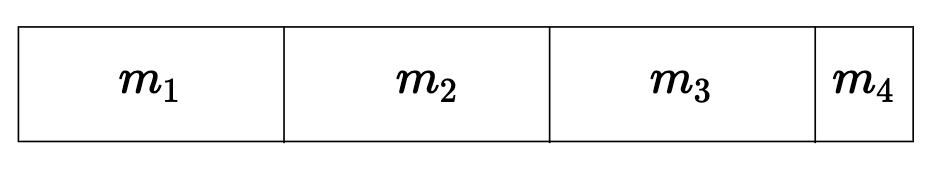
\includegraphics[scale=0.4]{img/cap5/4.png}
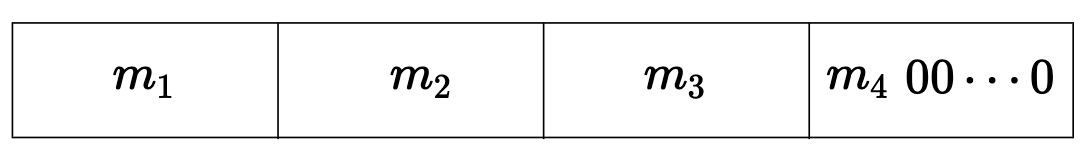
\includegraphics[scale=0.4]{img/cap5/5.png}
\end{figure}

Sin embargo, esta no es una buena idea ya que es fácil encontrar colisiones: $h(m) = h(m0)$ si $|m|$ no es divisible por 128. Entonces, ¿qué debe cumplir una buena función de padding? Consideremos una función $Pad(\cdot)$ para bloques de largo $n$, por ejemplo, $n = 128$. Dado un mensaje $m \in \{0,1\}^*$, se debe tener que
$$
|Pad(m)| \geq n \quad \text{y} |Pad(m)| \quad \text{ es divisible por } n
$$
Los axiomas fundamentales del padding son:
\begin{itemize}
    \item $m$ es un prefijo de $Pad(m)$.
    \item si $|m_1| = |m_2|$, entonces $|Pad(m_1)| = |Pad(m_2)|$.
    \item si $|m_1| \neq |m_2|$, entonces el último bloque de $Pad(m_1)$ es distinto del último bloque de $Pad(m_2)$/
\end{itemize}
Si un padding cumple con estos axiomas, entonces $Pad$ es una \textbf{función inyectiva}. Si suponemos que $m_1 \neq m_2$, entonces:
\begin{itemize}
    \item si $|m_1| \neq |m_2|$, entonces $Pad(m_1) \neq Pad(m_2)$ ya que el último bloque de $Pad(m_1)$ es distinto del último bloque de $Pad(m_2)$.
    \item si $|m_1| = |m_2|$, entonces $Pad(m_1) \neq Pad(m_2)$ ya que $m_1$ es prefijo de $Pad(m_1)$ y $m_2$ es prefijo de $Pad(m_2)$.
\end{itemize}

\subsection{Construcción de Merkle-Damgård}
Juntando todo lo anterior, supongamos dados:
\begin{itemize}
    \item La función de compresión $(\gen, h')$ de Davies-Meyer.
    \item Para cada $n \in \mathbb{N}$, una función de padding $Pad_n$, que considera bloques con $n$ elementos y satisface los axiomas fundamentales.
\end{itemize}
Vamos a definir una función de hash $(\gen, h)$ para mensajes de largo arbitrario. Consideremos un parámetro de seguridad $1^n$, entonces, tenemos que $\gen(1^n) = s$ y luego $h^s:\{0,1\}^* \to \{0,1\}^n$. \medbreak

El valor del vector de inicialización $H_0$ está contenido en $s$, ya que $s$ puede ser definido como $(n, H_0)$. Luego, dado un $m \in \{0,1\}^*$, calculamos $h^s(m)$ de la siguiente forma:
\begin{enumerate}
    \item Supongamos que $Pad_n(m) = m_1 m_2 \cdots m_\ell$, donde el largo de cada bloque $m_i$ es $n$.
    \item Para cada $i \in \{1, \ldots, \ell\}$: $H_i = (h')^n(m_1 || H_{i-1})$
    \item $h^s(m) = H_\ell$
\end{enumerate}

Esta construcción $(\gen, h)$ es resistente a colisiones. Queda como ejercicio propuesto al lector demostrar esta afirmación, dado que $(\gen', h')$ es resistente a colsiones y cada función de padding $Pad_n$ satisface los axiomas fundamentales. Notar que:
\begin{itemize}
    \item Podemos reemplazar la construcción de Davies-Meyer por cualquier función de compresión resistente a colisiones.
    \item Podemos considerar funciones de compresión de la forma $h':\{0,1\}^{p(n)} \to \{0,1\}^n$, con $p(n)$ un polinomio tal que $p(n) > n$.
\end{itemize}

Pero, ¿qué función de padding usamos? Consideramos bloques de largo $n$:
\begin{figure}[H]
    \centering
    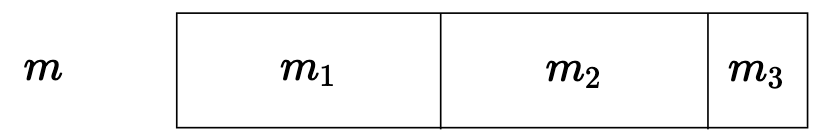
\includegraphics[scale=0.35]{img/cap5/6.png}
    \hspace{1.51cm}
    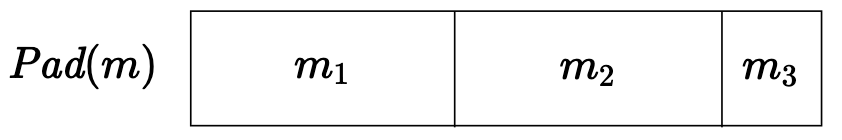
\includegraphics[scale=0.35]{img/cap5/7.png}
    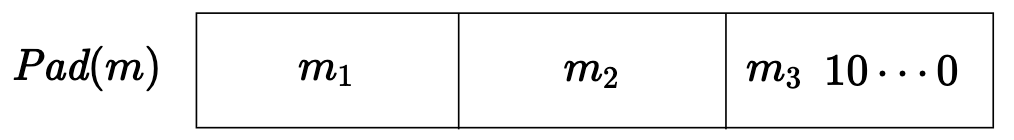
\includegraphics[scale=0.35]{img/cap5/8.png}
    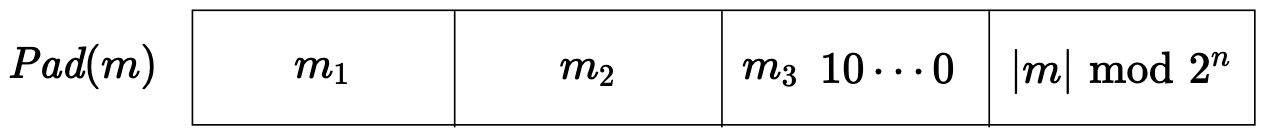
\includegraphics[scale=0.35]{img/cap5/9.png}
\end{figure}

Esta función de padding satisface los dos primeros axiomas fundamentales, pero pueden existir mensajes $m_1$ y $m_2$ tales que $|m_1| \neq |m_2|$ y los últimos bloques de $m_1$ y $m_2$ son iguales. Se debe tener que: $|m_1| \equiv |m_2| \bmod 2^n$, ya que si $|m_1| < |m_2|$, entonces $|m_2| > 2^n$. \medbreak

Si $n = 128$, entonces $|m_2| > 2^{128}$, y $m_2$ debe tener al menos $10^{38}$ dígitos. ¿Es posible escribir un número de este tamaño? \textbf{No.} Cisco estima que el tráfico de Internet en 2025 será de 175 zettabytes, vale decir, $175 \cdot 10^{21}$ bytes.

\subsection{Secure Hash Algorithm 2 (SHA-2)}
SHA-2 es una familia de funciones de funciones de hash.
\begin{itemize}
    \item Se definen utilizando la construcción de Merkle-Damgård
    \item Las funcoines de compresión son definidas utilizando la construcción de Davies-Meyer sobre un block cipher propio (no el de AES).
\end{itemize}
Por ejemplo, en SHA-256, el número se refiere al largo del hash. Esta función es una función de $\{0,1\}^*$ a $\{0,1\}^{256}$. SHA-256 puede considerarse como el resultado de instanciar el parámetro de seguridad el el valor 256 (de hecho, se usa en Bitcoin). También son utilizados otros ejemplos como SHA-224, SHA-384 y SHA-512. 

\paragraph{SHA-256.} Considera bloques de 512 bits, y sus estados internos $H_i$ son de 256 bits. La función de compresión es de la forma:
$$
h':\{0,1\}^{512} \times \{0,1\}^{256} \to \{0,1\}^{256}
$$
La función de padding se define utilizando las ideas descritas en las secciones anteriores, pero reservando los últimos 64 bits para el largo del mensaje $m$. Se realizan los siguientes pasos sobre el mensaje $m$:
\begin{enumerate}
    \item Se agrega un símbolo 1.
    \item Se agregan $\ell$ símbolos 0, donde $\ell$ es el menor número natural tal que $|m| + 1 + \ell \equiv 448 \bmod 512$.
    \item Se agrega $|m| \bmod 2^{64}$.
\end{enumerate}
El vector de inicialización $H_0$ se define como $H_0^1H_0^2H_0^3H_0^4H_0^51H_0^61H_0^7H_0^8$, donde $H_0^i$ tiene los primeros 32 bits de la parte decimal de la raíz cuadrada del $i$-ésimo número primo. Por ejemplo, $H_0^1$ tiene los primeros 32 bits de la parte decimal de $\sqrt{2}$:
$$
H_0^1 = 01101010000010011110011001100111
$$

\subsection{HMAC}
HMAC, siglas en inglés correspondientes a \textit{Hash-based message authentication code}, corresponde a la construcción de un código de autentificación de mensajes $\mac$ en base a una función de hash $h$. ¿Qué pasa si definimos $\mac_k(m) = h(k || m)$? Recordemos el juego que definía un buen MAC:
\begin{enumerate}
    \item El verificador genera una llave $k$.
    \item El adversario envía $m_0 \in \ca{M}$.
    \item El verificador responde $\mac_k(m_0)$.
    \item Los pasos 2 y 3 se repiten tantas veces como quiera el adversario.
    \item El adversario envía $(m,t)$, siendo $m$ un mensaje que no se había enviado antes.
\end{enumerate}
El adversario gana si $\ver_k(m,t) = 1$. Ahora, pensemos que estamos usando SHA-2, ¿puede el adversario ganar el juego? Hagamos una simplificación, el largo de $k$ es un bloque:
\img{img/cap5/10.png}{0.4}
Donde:
\begin{itemize}
    \item $k \, m_0 \cdots m_\ell$ es en realidad $Pad(k||m)$.
    \item En particular, $m \neq m_0 \cdots m_\ell$. 
\end{itemize}
Entonces, ¿cómo se ve $Pad(Pad(k||m))$?
$$
Pad(Pad(k||m)) = k\,m_0 \cdots m_\ell \, m_{\ell + 1}
$$
Por lo tanto, el adversario puede calcular y ganar el juego:
\img{img/cap5/11.png}{0.4}

Donde $m' = m_0 \cdots m_\ell$. Este tipo de ataques se conoce como \textit{length extension attacks}. \medbreak

Si tratamos con $\mac_k(m) = h(m||k)$ (al revés del ejemplo anterior), no podemos hacer ataques de extensión de largo, pero si puede ocurrir una colisión de dos mensajes del mismo largo, que termina rompiendo el MAC.
\img{img/cap5/12.png}{0.4}

Podemos seguir tratando varias funciones de hash, pero lo que podemos \textit{intuir} que es seguro es
$$
\mac_k(m) = h(k_2 \mid\mid h(k_1 \mid\mid m))
$$
donde $k_1$ y $k_2$ ocupan exclusivamente un bloque, son distintas, se derivan de forma determinista a partir de $k$ y no se pueden obtener sin $k$. El estándar se define de la siguiente forma:
$$
k' = \begin{cases}
h(k) &k\text{ usa más de un bloque} \\
k &\text{e.o.c.}
\end{cases}
$$
Así, podemos definir a $\hmac$ como:
$$
\hmac_k(m) = h(k_2 \mid\mid h(k_1 \mid\mid m))
$$
\img{img/cap5/13.png}{0.4}

% \section{Extracción de información}

\subsection{Extracción}

Imaginemos que tenemos un log de la forma
$$
    \begin{array}{lll}
        \texttt{18:30} & \texttt{ ERROR 06} \\
        \texttt{19:10} & \texttt{ OK 00}    \\
        \texttt{20:00} & \texttt{ ERROR 19}
    \end{array}
$$
y queremos obtener todas las horas $\texttt{HH:MM}$, quizá con una expresión regular $R =$ ({\textbackslash}d{\textbackslash}d:{\textbackslash}d{\textbackslash}d). ¿Cómo podemos \textbf{automatizar} esta tarea de extraer datos?
\begin{enumerate}
    \item Una tarea como la anterior \textbf{se puede programar fácilmente}, ¿por qué queremos automatizarla?
    \item Las expresiones regulares ya hacen el trabajo anterior, ¿por qué queremos \textbf{estudiar este problema de nuevo}?
\end{enumerate}
En esta última sección veremos \textbf{nuevas técnicas formales y algorítmicas} para entender y resolver este problema.

\subsubsection{Spans}

\paragraph{Definición.} Para un documento $d = a_0 a_1 \ldots a_{n-1}$ se define un \textbf{span} $s$ de $d$ como:
\alignformula{
s=[i, j\rangle
}
tal que $0 \leq i \leq j \leq n$. \bigbreak

Si $s = [i,j \rangle$ es un span de $d$ se define:
\alignformula{
d[s]=d[[i, j\rangle]=a_i a_{i+1} \ldots a_{j-1}
}
como el \textbf{contenido del span} $s$ en $d$. Si $i = j$, entonces $d[[i, i\rangle]=\epsilon$.
\ejemplo{}{}{
    \vspace{-10pt}
    \img{img/cap6/ejemplo1.png}{0.4}
}

Denotamos el conjunto de \textbf{todos los spans} de $d$ como $\texttt{Spans}(d)$.

\newpage
\subsubsection{Regex}
\paragraph{Sintaxis.} Sea $\Sigma$ un alfabeto finito y $\ca{X}$ un conjunto de variables. $R$ es una expresión regular con variables (o \textbf{regex}) sobre $\Sigma$ si $R$ es igual a:
\begin{enumerate}
    \item $a$, para alguna letra $a \in \Sigma$.
    \item $\epsilon$
    \item $\mathbf{x}\{R_1\}$, donde $R_1$ es una regex y $\mathbf{x} \in X$.
    \item $(R_1 + R_2)$, donde $R_1$ y $R_2$ son regex.
    \item $(R_1 \cdot R_2)$, donde $R_1$ y $R_2$ son regex.
    \item $(R_1^*)$, donde $R_1$ es una regex.
\end{enumerate}

$\mbb{x}\{R_1\}$ representa que el \textbf{span capturado} por $R_1$ lo almacenaremos en la variable $\mbb{x}$.

\ejemplo{}{}{
    Sea $\Sigma = \{a,b,\sbar\}$.
    \begin{itemize}
        \item $\Sigma^* \cdot \mbb{x}\{abba\} \cdot \Sigma^*$
        \item $\Sigma^* \cdot \sbar \cdot \mbb{x}\{ab \cdot (a+b)^*\}\cdot \sbar \cdot \Sigma^*$
        \item $\Sigma^* \cdot \sbar \cdot \mbb{x}\{(a+b)^*\}\cdot \sbar \cdot \mbb{y}\{(a+b)^*\} \cdot \sbar \cdot \Sigma^*$
        \item $(\Sigma^* \cdot \sbar + \epsilon) \cdot \mbb{z}\{\mbb{x}\{(a+b)^+\}\cdot \sbar \cdot \mbb{y}\{(a+b)^+\}\} \cdot (\epsilon + \sbar \cdot \Sigma^*)$
        \item $\Sigma^* \cdot \mbb{x}\{abba\} \cdot \sbar \cdot \mbb{x}\{baba\} \cdot \Sigma^*$
    \end{itemize}
}

\paragraph{Regex válidas.} Sea $\texttt{Var}(R)$ el conjunto de \textbf{todas las variables} en $\ca{X}$ mencionadas en $R$. Decimos que $R$ es una regex \textbf{válida} si, y sólo si, todas las siguientes condiciones se cumplen:
\begin{enumerate}
    \item si $R = R_1 \cdot R_2$, entonces $\texttt{Var}(R_1) \cap \texttt{Var}(R_2) = \varnothing$, y $R_1$ y $R_2$ son válidas.
    \item si $R = R_1 + R_2$, entonces $\texttt{Var}(R_1) = \texttt{Var}(R_2)$, y $R_1$ y $R_2$ son válidas.
    \item si $R = R_1^*$, entonces $\texttt{Var}(R_1) = \varnothing$, y $R_1$ es válida.
    \item si $R = \mbb{x}\{R_1\}$, entonces $\mbb{x} \notin \texttt{Var}(R_1)$, y $R_1$ es válida.
\end{enumerate}

Si $R$ es \textbf{válida} nos permite asignar las variables de \textbf{manera correcta}.

\ejemplo{}{}{
    Las siguientes regex son válidas:
    \begin{itemize}
        \item $\Sigma^* \cdot \mbb{x}\{abba\} \cdot \Sigma^*$
        \item $\Sigma^* \cdot \mbb{x}\{abba\} \cdot \sbar \cdot \mbb{y}\{baba\} \cdot \Sigma^*$
        \item $\Sigma^* \cdot \sbar \cdot \mbb{x}\{ab\cdot (a+b)^*\} \cdot \sbar \cdot \Sigma^*$
    \end{itemize}
    Las siguientes regex \textbf{no} son válidas:
    \begin{itemize}
        \item $\Sigma^* \cdot \mbb{x}\{abba\} \cdot \sbar \cdot \mbb{x}\{baba\} \cdot \Sigma^*$
        \item $\Sigma^* \cdot (\mbb{x}\{abba\} + \mbb{y}\{baba\}) \cdot \Sigma^*$
        \item $\Sigma^* \cdot \sbar \cdot (\mbb{x}\{ab \cdot (a+b)^*\} \cdot \sbar)^* \cdot \Sigma^*$
    \end{itemize}
}

\paragraph{Mappings.} Un \textbf{mapping} de $R$ sobre un documento $d \in \Sigma^*$ es una función:
\alignformula{
    \mu: \texttt{Var}(R) \to \texttt{Spans}(d)
}

donde el dominio de $\mu$ es $\texttt{dom}(\mu) = \texttt{Var}(R)$. \bigbreak

Se define el mapping $\mu = \, \perp$ como el \textbf{mapping vacío} donde $\texttt{dom}(\perp) = \varnothing$.

\ejemplo{}{}{
    \img{img/cap6/ejemplo4.png}{0.3}
}

\begin{itemize}
    \item Para una variable $\mbb{x}$ y span $s$ se define el \textbf{mapping} de una variable:
          $$
              \mu=[\mathbf{x} \mapsto s] \quad \text { tal que } \quad \texttt{dom}(\mu)=\{\mathbf{x}\} \quad \text { y } \quad \mu(\mathbf{x})=s
          $$

    \item Para $k \in \mathbb{N}$ se define el \textbf{mapping} $\mu + k$ tal que $\texttt{dom}(\mu + k) = \texttt{dom}(\mu)$ y:
          $$
              \text{si } \mu(\mathbf{x})=[i, j\rangle \text { entonces }[\mu+k](\mathbf{x})=[i+k, j+k\rangle \text {.}
          $$

    \item Para mappings $\mu_1,\mu_2$ con $\texttt{dom}(\mu_1) \cap \texttt{dom}(\mu_2) = \varnothing$ se define la \textbf{unión}:
          $$
              \mu=\mu_1 \cup \mu_2 \quad \text { tal que } \quad \mu(\mathbf{x})= \begin{cases}
                  \mu_1(\mathbf{x}) & \text { si } \mathbf{x} \in \operatorname{dom}\left(\mu_1\right) \\
                  \mu_2(\mathbf{x}) & \text { si } \mathbf{x} \in \operatorname{dom}\left(\mu_2\right)
              \end{cases}
          $$
\end{itemize}

\paragraph{Semántica regex.} Para una regex válida $R$ cualquiera, se define la función $\llbracket R \rrbracket$ \textbf{inductivamente} sobre documentos $d \in \Sigma^*$:
\begin{enumerate}
    \item $\llbracket a \rrbracket(d)=\{\perp\}$ si $d = a$, y $\varnothing$ en otro caso.
    \item $\llbracket \epsilon \rrbracket(d)=\{\perp\}$ si $d = \epsilon$, y $\varnothing$ en otro caso.
    \item $\llbracket \mathbf{x}\left\{R_1\right\} \rrbracket(d)=\left\{\mu \cup[\mathbf{x} \mapsto s] \mid \mu \in \llbracket R_1 \rrbracket(d) \text { y } s=[0,|d|\rangle\right\}$
    \item $\llbracket R_1 \cdot R_2 \rrbracket(d)=\left\{\begin{array}{l|l}
                  \mu_1 \cup\left(\mu_2+\left|d_1\right|\right) & \begin{array}{l}
                                                                      \text { existe } d_1, d_2 \text { tal que } d=d_1 \cdot d_2, \\
                                                                      \mu_1 \in \llbracket R_1 \rrbracket\left(d_1\right) \text { y } \mu_2 \in \llbracket R_2 \rrbracket\left(d_2\right)
                                                                  \end{array}
              \end{array}\right\}$

          Como $R_1 \cdot R_2$ son válidas, entonces sabemos que $\texttt{dom}(\mu_1) \cap \texttt{dom}(\mu_2) = \varnothing$.

    \item $\llbracket R_1+R_2 \rrbracket(d)=\llbracket R_1 \rrbracket(d) \cup \llbracket R_2 \rrbracket(d)$

    \item $\llbracket R_1^* \rrbracket(d)=\bigcup_{k=0}^{\infty} \llbracket\left(R_1\right)^k \rrbracket(d)$

          Como $\texttt{Var}(R_1) = \varnothing$, entonces $\llbracket R_1^* \rrbracket(d)=\{\perp\}$ si, y sólo si, $d \in \mathcal{L}\left(R_1^*\right)$.
\end{enumerate}

\ejemplo{}{}{
    \begin{itemize}
        \item $\llbracket b \rrbracket(a) = \varnothing$
        \item $\llbracket b \rrbracket(b) = \{\perp\}$
        \item $\llbracket \mbb{x}\{b\} \rrbracket(a) = \varnothing$
        \item $\llbracket \mbb{x}\{b\} \rrbracket(b) = \{ [\mbb{x} \mapsto [0,1\rangle] \}$
        \item $\llbracket \mathbf{x}\{b\} b \rrbracket(b b)=\{[\mathbf{x} \mapsto[0,1\rangle]\}$
        \item $\llbracket b \mathbf{x}\{b\}\rrbracket(b b)=\{[\mathbf{x} \mapsto[1,2\rangle]\}$
        \item $\llbracket\mathbf{x}\{b\} \mathbf{y}\{b\}\rrbracket(b b)=\{[\mathbf{x} \mapsto[0,1\rangle, \mathbf{y} \mapsto[1,2\rangle]\}$
        \item $\llbracket\mathbf{x}\{b\} b+b \mathbf{x}\{b\}\rrbracket(b b)=\{[\mathbf{x} \mapsto[0,1\rangle],[\mathbf{x} \mapsto[1,2\rangle]\}$
    \end{itemize}
}

\ejemplo{}{}{
    \vspace{-10pt}
    \img{img/cap6/ejemplo6.png}{0.5}

    \begin{itemize}

        \item $\llbracket\Sigma^* \cdot \mathbf{x}\{a b a+b a b\} \cdot \Sigma^*\rrbracket(d)=\{[\mathbf{x} \mapsto[10,13\rangle],[\mathbf{x} \mapsto[11,14\rangle]\}$

        \item $\llbracket\Sigma^* \cdot \sbar \cdot \mathbf{x}\left\{b a \cdot(a+b)^*\right\} \cdot \sbar \cdot \Sigma^*\rrbracket(d)=\{[\mathbf{x} \mapsto[7,9\rangle],[\mathbf{x} \mapsto[10,14\rangle]\}$

        \item $\llbracket\Sigma^* \cdot \mathbf{x}\{a b b a\} \cdot \sbar \cdot \mathbf{y}\{b a\} \cdot \Sigma^*\rrbracket(d)=\{[\mathbf{x} \mapsto[2,6\rangle, \mathbf{y} \mapsto[7,9\rangle]\}$

        \item $\llbracket\Sigma^* \cdot \sbar \cdot \mathbf{x}\left\{(a+b)^*\right\} \cdot \sbar \cdot \mathbf{y}\left\{(a+b)^*\right\} \cdot \sbar \cdot \Sigma^*\rrbracket(d)=\{[\mathbf{x} \mapsto[2,6\rangle, \mathbf{y} \mapsto[7,9\rangle],[\mathbf{x} \mapsto[7,9\rangle, \mathbf{y} \mapsto[10,14\rangle]\}$

        \item $\llbracket\Sigma^* \cdot \mathbf{x}\left\{\Sigma^*\right\} \cdot \Sigma^* \rrbracket(d)=\texttt{Spans}(d)$

    \end{itemize}
}

\paragraph{Evaluación regex.} Podemos preguntarnos:

\begin{itemize}
    \item Dado una regex $R$ con una variable, ¿de qué tamaño puede ser $|\llbracket R \rrbracket(d)|$ con respecto a $|d|$ \textbf{en el peor caso}?
    \item Dado una regex $R$ con $k$ variables, ¿de qué tamaño puede ser $|\llbracket R \rrbracket(d)|$ con respecto a $|d|$ y $k$ \textbf{en el peor caso}?
\end{itemize}

La respuesta es que el tamaño de $|\llbracket R \rrbracket(d)|$ puede crecer de manera exponencial. ¿Cómo podemos evaluar entonces una regex de $R$ \textbf{eficientemente}? Analizamos una herramienta para lograr esto a continuación.

\subsubsection{Vset autómata}

¿Qué tiene de nuevo un autómata con variables (vset autómata)?
\begin{enumerate}
    \item Tiene transiciones con \textbf{abre} y \textbf{cierra} de variable $\mbb{x}$:
          \alignformula{
              p \stackrel{\langle x}{\rightarrow} q \quad y \quad p \stackrel{x\rangle}{\rightarrow} q
          }
    \item Cada ejecución define un \textbf{mapping} de las variables a spans.
\end{enumerate}
Un \textbf{vset autómata} será nuestro primer modelo para \textbf{compilar regex}.

\paragraph{Definición.} Un vset autómata (VA) es una tupla:
\alignformula{
    \ca{A} = (Q, \Sigma, \ca{X}, \Delta, I, F)
}
\begin{itemize}
    \item $Q$ es un conjunto finito de estados.
    \item $\Sigma$ es el alfabeto de input.
    \item $\ca{X}$ es un conjunto finito de variables.
    \item $\Delta \subseteq Q \times(\Sigma \cup\{\epsilon\} \cup\{\langle\mathbf{x}, \mathbf{x}\rangle \mid \mathbf{x} \in \mathcal{X}\}) \times Q$ es la relación de transición.
    \item $I \subseteq Q$ es un conjunto de estados iniciales.
    \item $F \subseteq Q$ es el conjunto de estados finales (o aceptación).
\end{itemize}

`$\langle \mbb{x}$' simboliza \textbf{abrir} y `$\mbb{x}\rangle$' simboliza \textbf{cerrar} la variable $\mbb{x}$.

\ejemplo{vset autómatas}{}{
    \begin{figure}[H]
        \centering
        \includegraphics[scale=0.45]{img/cap6/ejemplo7_1.png}
        \includegraphics[scale=0.45]{img/cap6/ejemplo7_2.png}
        \includegraphics[scale=0.45]{img/cap6/ejemplo7_3.png}
    \end{figure}
}

\paragraph{Ejecución.} Sea $\ca{A} = (Q,\Sigma,\ca{X},\Delta,I,F)$ un VA y $d = a_0 \ldots a_{n-1} \in \Sigma^*$ un documento. Tenemos que:
\begin{itemize}
    \item Un par $(p, i) \in Q \times\{0, \ldots, n\}$ es una \textbf{configuración} de $\ca{A}$ sobre $d$.
    \item Una configuración $(p,0)$ es \textbf{inicial} si $q \in I$.
    \item Una configuración $(p, |d|)$ es \textbf{final} si $q \in F$.
\end{itemize}
\textit{``Intuitivamente, una configuración $(p,i)$ representa que $\ca{A}$ se encuentra en el estado $p$ antes de leer $a_i$''.} \bigbreak

Una \textbf{ejecución} (o \textit{run}) $\rho$ de $\ca{A}$ sobre $d$ es una secuencia:
\alignformula{
    \rho:\left(p_0, i_0\right) \stackrel{o_1}{\rightarrow}\left(p_1, i_1\right) \stackrel{o_2}{\rightarrow} \ldots \stackrel{o_m}{\rightarrow}\left(p_m, i_m\right)
}
tal que cumple todas las siguientes condiciones:
\begin{itemize}
    \item $o_k \in \Sigma \cup\{\epsilon\} \cup\{\langle\mathbf{x}, \mathbf{x}\rangle \mid \mathbf{x} \in \mathcal{X}\}$ con $k \leq m$,
    \item $(p_0, i_0)$ es una configuración inicial,
    \item para todo $k < m$, $\left(p_k, o_{k+1}, p_{k+1}\right) \in \Delta$,
    \item para todo $k \leq m$, si $o_k \in \Sigma$, entonces $o_k = a_{i_{k-1}}$ y $i_k = i_{k-1} + 1$,
    \item para todo $k \leq m$, si $o_k \in\{\epsilon\} \cup\{\langle\mathbf{x}, \mathbf{x}\rangle \mid \mathbf{x} \in \mathcal{X}\}$, entonces $i_k = i_{k-1}$.
\end{itemize}

Una ejecución $\rho$ es de \textbf{aceptación} si $(p_m, i_m)$ es de aceptación.

\ejemplo{Ejecuciones}{}{
    \img{img/cap6/ejemplo8.png}{0.5}
    Algunas ejecuciones sobre $d$:
    \begin{itemize}
        \item $\rho_1:\left(p_0, 0\right) \stackrel{a}{\rightarrow}\left(p_0, 1\right) \stackrel{b}{\rightarrow}\left(p_0, 2\right) \stackrel{a}{\rightarrow}\left(p_0, 3\right)$
        \item $\rho_2:\left(p_0, 0\right) \stackrel{a}{\rightarrow}\left(p_0, 1\right) \stackrel{\epsilon}{\rightarrow}\left(p_1, 1\right) \stackrel{\langle x}{\rightarrow}\left(p_2, 1\right) \stackrel{b}{\rightarrow}\left(p_2, 2\right) \stackrel{\mathrm{x}\rangle}{\rightarrow}\left(p_3, 2\right) \stackrel{a}{\rightarrow}\left(p_3, 3\right)$
        \item $\rho_3:\left(p_0, 0\right) \stackrel{a}{\rightarrow}\left(p_0, 1\right) \stackrel{\langle x}{\rightarrow}\left(p_2, 1\right) \stackrel{b}{\rightarrow}\left(p_2, 2\right) \stackrel{\mathrm{x}\rangle}{\rightarrow}\left(p_3, 2\right) \stackrel{a}{\rightarrow}\left(p_3, 3\right)$
        \item $\rho_4:\left(p_0, 0\right) \stackrel{a}{\rightarrow}\left(p_0, 1\right) \stackrel{\langle x}{\rightarrow}\left(p_2, 1\right) \stackrel{b}{\rightarrow}\left(p_2, 2\right) \stackrel{\langle x}{\rightarrow}\left(p_3, 2\right) \stackrel{a}{\rightarrow}\left(p_3, 3\right)$
    \end{itemize}

    Donde $\rho_2$ y $\rho_3$ son ejecuciones válidas.
}

Una ejecución $\rho$ es \textbf{válida} si, y sólo si, para todo $\mbb{x} \in \ca{X}$:
\begin{itemize}
    \item existe un único $k_1 \leq m$ tal que $o_{k_1} = \mbb{\langle x}$,
    \item existe un único $k_2 \leq m$ tal que $o_{k_2} = \mbb{x\rangle}$ y
    \item $k_1 < k_2$.
\end{itemize}

\textit{``Intuitivamente, $\rho$ es válida si, y sólo si, todas las variables se abren y cierran correctamente.''} \bigbreak

Si $\rho$ es \textbf{válida} se define el \textbf{mapping de} $\rho$ $\texttt{map}(\rho): \ca{X} \to \texttt{Spans}(d)$ tal que:
\alignformula{
[\texttt{map}(\rho)](\mathbf{x})=\left[i_{k_1}, i_{k_2}\right\rangle
}
para todo $\mbb{x} \in \ca{X}$ y $k_1,k_2 \leq m$ con $i_{k_1} = \langle \mbb{x}$ y $i_{k_2} = \mbb{x}\rangle$.

\ejemplo{Mappings de $\rho$}{}{
El mapping para las ejecuciones válidas del ejemplo anterior es:
$$
    \texttt{map}\left(\rho_2\right)=\texttt{map}\left(\rho_3\right)=[\mathbf{x} \mapsto[1,2\rangle]
$$
}

\paragraph{Función de extracción.} Sea $\ca{A}$ un VA. Se define la función $\llbracket \mathcal{A} \rrbracket$ tal que para todo documento $d \in \Sigma^*$:
\alignformula{
    \llbracket \mathcal{A} \rrbracket(d)=\{ \texttt{map}(d) \mid \rho \text{ es una ejecución válida y de aceptación de } \ca{A} \text{ sobre } d\}
}

Un VA nos entrega otra forma de extraer información de un documento.

\subsubsection{Desde regex a VA}

\paragraph{Definición.} Sea $\ca{A}$ un VA. Decimos que $\ca{A}$ es \textbf{funcional} si, y sólo si, para todo documento $d$ y para toda ejecución $\rho$ de $\ca{A}$ sobre $d$:
\alignformula{
    \text{si } \rho \text{ es de aceptación, entonces } \rho \text{ es válida.}
}

Para funcional solo necesitamos verificar que la ejecución es de aceptación.

\teorema{}{}{
Para toda regex $R$ válida, existe un vset autómata \textbf{funcional} $\ca{A}_R$ de \textbf{tamaño lineal} en $|R|$ tal que para todo documento $d$:
$$
    \llbracket R \rrbracket(d)=\llbracket \mathcal{A}_{\mathcal{R}} \rrbracket(d)
$$
}
La demostración de este teorema queda como ejercicio propuesto al lector (es similar al Teorema de Kleene).

\subsection{Enumeración de resultados: Autómatas con anotaciones}

Veamos el siguiente problema:
\begin{table}[H]
    \centering
    \begin{tabular}{ll}
        $\texttt{PROBLEMA:}$ & Evaluación de regex                                         \\
        $\texttt{INPUT:}$    & Una regex $R$ y                                             \\
                             & un documento $w$                                            \\
        $\texttt{OUTPUT:}$   & Enumerar todos los mappings en $\llbracket R \rrbracket(d)$
    \end{tabular}
\end{table}
La idea es:
\begin{enumerate}
    \item Transformamos $R$ a un vset autómata $\ca{A}_R$.
    \item Enumeramos los resultados $\llbracket \mathcal{A}_R \rrbracket(d)$.
\end{enumerate}
¿Cómo computamos todos los mappings en $\llbracket \mathcal{A}_R \rrbracket(d)$? ¿Cómo los encontramos si son demasiados? Veamos qué podemos hacer.

\subsubsection{Representación de mappings}
Sea $d = a_0 \ldots a_{n-1}$, un conjunto de variables $\ca{X}$ y un mapping $\mu: \ca{X} \to \texttt{Spans}(d)$.

\paragraph{Definiciones.} Tenemos que:
\begin{enumerate}
    \item Se define el \textbf{conjunto de marcas de} $\ca{X}$ como:
          \alignformula{
              \texttt{Markers}(\mathcal{X})=\{\langle\mathbf{x}\mid \mathbf{x} \in \mathcal{X}\} \cup\{\mathbf{x}\rangle \mid \mathbf{x} \in \mathcal{X}\}
          }
    \item Se define el \textbf{mapping inverso} de $\mu$ como $\mu^{\text {inv }}:[0, n] \rightarrow 2^{\operatorname{Markers}(\mathcal{X})}$:
          \alignformula{
          \left.\mu^{\text {inv }}(i)=\{\langle\mathbf{x} \mid\exists j.\ \mu(\mathbf{x})=[i, j\rangle \in \mathcal{X}\} \cup\{\mathbf{x}\rangle \mid \exists j.\ \mu(\mathbf{x})=[j, i\rangle \in \mathcal{X}\right\}
          }
    \item Se define la \textbf{secuenciación} de $\mu$ como $\texttt{seq}(\mu) = \texttt{seq}_0(\mu) \cdot \ldots \cdot \texttt{seq}_n(\mu)$:
          \alignformula{
              \texttt{seq}_i(\mu)= \begin{cases}\left(i, \mu^{\mathrm{inv}}(i)\right) & \mu^{\mathrm{inv}}(i) \neq \varnothing \\ \epsilon & \mu^{\mathrm{inv}}(i)=\varnothing\end{cases}
          }

          $\texttt{seq}(\mu)$ es una \textbf{representación equivalente} de un mapping $\mu$, y nos será más conveniente para nuestros algoritmos de enumeración de resultados.
\end{enumerate}

\ejemplo{}{}{
    \vspace{-10pt}
    \img{img/cap6/ejemplo10.png}{0.425}
    $$
        \texttt{seq}(\mu)=(15,\{\langle\mathbf{x},\langle\mathbf{z}\})\ (20,\{\mathbf{x}\rangle\})\ (24,\{\langle\mathbf{y}\})\ (26,\{\mathbf{y}\rangle, \mathbf{z}\rangle\})
    $$
}

\subsubsection{Autómatas con anotaciones}
\paragraph{Definición.} Un autómata con anotaciones (AnnA) es una tupla:
\alignformula{
    \ca{N}=(Q, \Sigma, \Lambda, \Delta, I, F)
}
\begin{itemize}
    \item $Q$ es un conjunto finito de estados.
    \item $\Sigma$ es el alfabeto de input.
    \item $\Lambda$ es un conjunto finito de etiquetas (Labels).
    \item $\Delta \subseteq Q \times(\Sigma \cup \Sigma \times \Lambda) \times Q$ es la relación de transición.
    \item $I \subseteq Q$ es un conjunto de estados iniciales.
    \item $F \subseteq F$ es el conjunto de estados finales (o aceptación).
\end{itemize}

Las transiciones $(p,a,l,q)$ simbolizan que al leer la letra $a$, esta letra \textbf{será anotada} con $l$.
\ejemplo{}{}{
    \begin{figure}[H]
        \centering
        \includegraphics[scale=0.5]{img/cap6/ejemplo11_1.png}
        \includegraphics[scale=0.5]{img/cap6/ejemplo11_2.png}
    \end{figure}
}

\paragraph{Ejecución.} Sea un AnnA $\ca{N} = (Q, \Sigma, \Lambda, \Delta, I, F)$ y un documento $d = a_0 \ldots a_{n-1} \in \Sigma^*$. Una \textbf{ejecución} $\rho$ de $\ca{N}$ sobre $d$ es una secuencia:
$$
    \rho: p_0 \stackrel{t_0}{\rightarrow} p_1 \stackrel{t_1}{\rightarrow} \ldots \stackrel{t_{n-1}}{\rightarrow} p_n
$$
tal que cumple todas las siguientes condiciones:
\begin{enumerate}
    \item $p_0 \in I$
    \item para todo $i < n$, $t_i$ es de la forma $t_i = a_i$ o $t_i = (a_i, l)$ para algún $l \in \Lambda$
    \item para todo $i < n$, $(p_i, t_i, p_{i+1}) \in \Delta$
\end{enumerate}

Se define la \textbf{anotación de} $\rho$ como $\texttt{ann}(\rho) = \texttt{ann}_0(t_0) \cdot \ldots \cdot \texttt{ann}_n(t_{n-1})$:
$$
    \texttt{ann}_i(t)= \begin{cases}(i, l) & t=(a, l) \\ \epsilon & t=a\end{cases}
$$
Decimos que $\rho$ es de \textbf{aceptación} si, y sólo si, $q_n \in F$.

\ejemplo{Ejecuciones}{}{
    \vspace{-10pt}
    \img{img/cap6/ejemplo12.png}{0.55}

    Algunas ejecuciones sobre $d$:
    \begin{itemize}

        \item $\rho_1: p_0 \stackrel{a}{\rightarrow} p_0 \stackrel{\sbar / \langle}{\rightarrow} p_1 \stackrel{a / \bullet}{\rightarrow} p_1 \stackrel{b}{\rightarrow} p_1 \stackrel{b}{\rightarrow} p_1 \stackrel{a / \bullet }{\rightarrow} p_1 \stackrel{\sbar / \rangle}{\rightarrow} p_2 \stackrel{b}{\rightarrow} p_2 \stackrel{a}{\rightarrow} p_2 \stackrel{\hphantom{a}\sbar\hphantom{a}}{\rightarrow} p_2 \stackrel{b}{\rightarrow} p_2$

        \item $\rho_2: p_0 \stackrel{a}{\rightarrow} p_0 \stackrel{\hphantom{a}\sbar\hphantom{a}}{\rightarrow} p_0 \stackrel{a}{\rightarrow} p_0 \stackrel{b}{\rightarrow} p_0 \stackrel{b}{\rightarrow} p_0 \stackrel{a}{\rightarrow} p_0 \stackrel{\sbar / \langle}{\rightarrow} p_1 \stackrel{b}{\rightarrow} p_1 \stackrel{a / \bullet}{\rightarrow} p_1 \stackrel{\sbar / \rangle}{\rightarrow} p_2 \stackrel{b}{\rightarrow} p_2$
    \end{itemize}
    Además, tenemos que:
    \begin{itemize}
        \item $\texttt{ann}\left(\rho_1\right)=(1,\langle)(2, \bullet)(5, \bullet)(6,\rangle) \qquad \qquad a \, \overset{\langle}{\sbar} \, \overset{\bullet}{a}\, b\, b\, \overset{\bullet}{a}\, \overset{\rangle}{\sbar}\, b\, a\, \sbar \, b$

        \item $\texttt{ann}\left(\rho_2\right)=(6,\langle)(8, \bullet)(9,\rangle) \qquad \qquad \qquad a \, \sbar \, a \, b \, b \, a \, \overset{\langle}{\sbar} \, b \, \overset{\bullet}{a} \, \overset{\rangle}{\sbar} \, b $
    \end{itemize}
}

\paragraph{Output de un AnnA.} Sea $\ca{N}$ un AnnA. Se define la función $\llbracket \mathcal{N} \rrbracket$ tal que para todo documento $d \in \Sigma^*$:
\alignformula{
    \llbracket\mathcal{N} \rrbracket(d)=\{\texttt{ann}(\rho) \mid \rho \text { es una ejecución aceptación de } \mathcal{N} \text { sobre } d\}
}

\newpage

\ejemplo{Output de un AnnA}{}{
    \vspace{-10pt}
    \img{img/cap6/ejemplo12.png}{0.55}

    Para el documento $d$ se tiene que:
    $$
        \llbracket\mathcal{N}\rrbracket(d)=\{(1,\langle)(2, \bullet)(5, \bullet)(6,\rangle),(6,\langle)(8, \bullet)(9,\rangle)\}
    $$
}

\subsubsection{Desde un vset a AnnA}

\teorema{}{}{
    Sea $\Sigma$ un alfabeto finito. Para todo vset autómata funcional $\ca{A}$ sobre $\Sigma$, existe un AnnA $\ca{N}$ sobre $\Sigma \cup \{\#\}$ tal que para todo documento $d$ sobre $\Sigma$:
    $$
        \llbracket\mathcal{N} \rrbracket(d \cdot \#)=\{\operatorname{seq}(\mu) \mid \mu \in \llbracket \mathcal{A} \rrbracket(d)\}
    $$
}

El teorema anterior nos dice que $\ca{N}$ entrega la \textbf{secuenciación} de los mappings en $\llbracket \mathcal{A} \rrbracket(d)$.

\paragraph{Propiedades.} Sea $\ca{A} = (Q, \Sigma, \ca{X}, \Delta, I, F)$ un vset autómata funcional y $p,q \in Q$. \textbf{Sin pérdida de generalidad}, desde ahora supondremos que todos los estados de un vset autómata funcional $\ca{A}$ son \textbf{útiles}. En otras palabras, para todo estado $p \in Q$ de $\ca{A}$:
\begin{itemize}
    \item Existe una ejecución (camino de transiciones) desde $I$ a $p$.
    \item Existe una ejecución (camino de transiciones) desde $p$ a $F$.
\end{itemize}

\paragraph{Definición.} Una \textbf{ejecución sin lectura} (ejec-SL) de $p$ a $q$ en $\ca{A}$ es una secuencia:
$$
    \pi: \quad p_0 \stackrel{s_0}{\rightarrow} p_1 \stackrel{s_1}{\rightarrow} \ldots \stackrel{s_{k-1}}{\rightarrow} p_k
$$
donde:
\begin{itemize}
    \item $p_0 = p$ y $p_k = q$
    \item para todo $i < k$, $(p_i, s_i, p_{i+1})$ y $s_i \in \texttt{Markers}(\ca{X}) \cup \{\epsilon\}$.
\end{itemize}

Una ejecución sin lectura es un \textbf{camino de transiciones} de $p$ a $q$ tal que $s_i \notin \Sigma$. También, definimos el \textbf{conjunto de} $\pi$ como
$$
    \texttt{set}(\pi) = \{ s_i \mid s_i \in \texttt{Markers}(\ca{X})\}
$$

\paragraph{Propiedades ejec-SL.} Tenemos que:
\begin{enumerate}
    \item Para todo $i \neq j$, si $s_i = s_j$, entonces $s_i = s_j = \epsilon$.
    \item Para todo par de ejec-SL distintas $\pi_1, \pi_2$ de $p$ a $q$ en $\ca{A}$, se cumple que $\texttt{set}(\pi_1) = \texttt{set}(\pi_2)$.
\end{enumerate}

La demostraciones de estas propiedades queda como ejercicio propuesto para el lector.

\newpage

\paragraph{Demostración teorema 33.} Dado un vset autómata funcional $\ca{A} = (Q, \Sigma, \ca{X}, \Delta, I, F)$, construimos:
$$
    \mathcal{N}=\left(Q, \Sigma \cup\{\#\}, 2^{\texttt{Markers }(\mathcal{X})}, \Delta^{\prime}, I, F\right)
$$
\begin{multicols}{2}
    $(p,a,q) \in \Delta'$ $\Leftrightarrow$ existe $p' \in Q$ y una ejec-SL $\pi$ de $p$ a $p'$ tal que $(p',a,q) \in \Delta$ y $\texttt{set}(\pi) = \varnothing$.
    \img{img/cap6/teo_1.png}{0.2}

    $(p,a,S,q) \in \Delta'$ $\Leftrightarrow$ existe $p' \in Q$ y ejec-SL $\pi$ de $p$ a $p'$ tal que $(p',a,q) \in \Delta$ y $\texttt{set}(\pi) = S \neq \varnothing$.
    \img{img/cap6/teo_2.png}{0.2}

    $(p,\#, q) \in \Delta'$ $\Leftrightarrow$ existe una ejec-SL $\pi$ de $p$ a $q$ tal que $\texttt{set}(\pi)=\varnothing$ y $q \in F$
    \img{img/cap6/teo_3.png}{0.2}

    $(p,\#, S, q) \in \Delta'$ $\Leftrightarrow$ existe una ejec-SL $\pi$ de $p$ a $q$ tal que $\texttt{set}(\pi)=S \neq \varnothing$ y $q \in F$
    \img{img/cap6/teo_4.png}{0.2}
\end{multicols}
Por las propiedades 1 y 2, la construcción es \textbf{correcta}. Por último, podemos ver que
$$
    \llbracket \mathcal{N} \rrbracket(d \cdot \#)=\{\texttt{seq}(\mu) \mid \mu \in \llbracket \mathcal{A} \rrbracket(d)\}
$$
\hfill $\blacksquare$

\ejemplo{Construcción}{}{
    \img{img/cap6/ejemplo14.png}{0.5}
}

\newpage

\subsubsection{Determinismo}

Sea $\ca{N} = (Q,\Sigma, \Lambda, \Delta, I, F)$ un autómata con anotaciones AnnA.

\paragraph{Definición.} Decimos que $\ca{N}$ es \textbf{Input-Output} determinista (I/O-determinista) si, y sólo si, $|I| = 1$ y para todo $\left(p, t_1, q_1\right),\left(p, t_2, q_2\right) \in \Delta$, si $t_1 = t_2$, entonces $q_1 = q_2$. \bigbreak

$\ca{N}$ funciona de manera determinista al recibir el documento y una \textbf{anotación simultáneamente}.

\ejemplo{}{}{
    \begin{figure}[H]
        \centering
        \includegraphics[scale=0.5]{img/cap6/ejemplo15_1.png}
        \includegraphics[scale=0.5]{img/cap6/ejemplo15_2.png}
    \end{figure}
}

\teorema{}{}{
Para todo AnnA $\ca{N} = (Q, \Sigma, \Lambda, \Delta, I, F)$, existe un AnnA I/O-determinista $\ca{N}^\text{det}$ tal que
$$
    \llbracket \mathcal{N} \rrbracket=\llbracket \mathcal{N}^{\text {det}} \rrbracket
$$
}

\paragraph{Demostración teorema 34.} Considere la determinización de $\ca{N}$ como:
$$
\mathcal{A}^{\text{det}}=\left(2^Q, \Sigma, \Lambda, \Delta^{\text{det}}, q_0^{\text{det}}, F^{\text{det}}\right)
$$
donde:
\begin{itemize}
    \item $2^Q=\{S \mid S \subseteq Q\}$ es el conjunto potencia de $Q$.
    \item $q_0^{\text{det}}=I$
    \item $\Delta^{\operatorname{det}}: 2^Q \times(\Sigma \cup \Sigma \times \Lambda) \rightarrow 2^Q$ tal que para todo $t \in \Sigma \cup(\Sigma \times \Lambda)$:
    $$
    \Delta^{\text{det}}(S, t)=\{q \in Q \mid \exists p \in S.\ (p, t, q) \in \Delta\}
    $$
    \item $F^{\text{det}}=\left\{S \in 2^Q \mid S \cap F \neq \varnothing\right\}$. \hfill $\blacksquare$
\end{itemize}











%----------------------------------------------------------------------------------------

\end{document}
